% ------------------------------------------------------------
% LaTeX Template für die DHBW zum Schnellstart!
% Original: https://github.wdf.sap.corp/vtgermany/LaTeX-Template-DHBW
% ------------------------------------------------------------
% ---- Präambel mit Angaben zum Dokument
\documentclass[
	fontsize=12pt,           % Leitlinien sprechen von Schriftgröße 12.
	paper=A4,
	twoside=false,
	listof=totoc,            % Tabellen- und Abbildungsverzeichnis ins Inhaltsverzeichnis
	bibliography=totoc,      % Literaturverzeichnis ins Inhaltsverzeichnis aufnehmen
	titlepage,               % Titlepage-Umgebung anstatt \maketitle
	headsepline,             % horizontale Linie unter Kolumnentitel
	abstract,              % Überschrift einschalten, Abstract muss in {abstract}-Umgebung stehen
]{scrreprt}                  % Verwendung von KOMA-Report
\usepackage[utf8]{inputenc}  % UTF8 Encoding einschalten
\usepackage[ngerman]{babel}  % Neue deutsche Rechtschreibung
% \usepackage[T1]{fontenc}     % Ausgabe von westeuropäischen Zeichen (auch Umlaute)
% \usepackage{fontspec}
\usepackage{microtype}       % Trennung von Wörtern wird besser umgesetzt
% \usepackage{lmodern}         % Nicht-gerasterte Schriftarten (bei MikTeX erforderlich)
\usepackage{graphicx}        % Einbinden von Grafiken erlauben
\usepackage{wrapfig}         % Grafiken fließend im Text
\usepackage{setspace}        % Zeilenabstand \singlespacing, \onehalfspaceing, \doublespacing
\usepackage[
	%showframe,                % Ränder anzeigen lassen
	left=2.7cm, right=2.5cm,
	top=2.5cm,  bottom=2.5cm,
	includeheadfoot,
	a4paper
]{geometry}                      % Seitenlayout einstellen
\usepackage{scrlayer-scrpage}    % Gestaltung von Fuß- und Kopfzeilen
\usepackage[printonlyused]{acronym}             % Abkürzungen, Abkürzungsverzeichnis
\usepackage{titletoc}            % Anpassungen am Inhaltsverzeichnis
\contentsmargin{0.75cm}          % Abstand im Inhaltsverzeichnis zw. Punkt und Seitenzahl
\usepackage[                     % Klickbare Links (enth. auch "nameref", "url" Package)
  hidelinks,                     % Blende die "URL Boxen" aus.
  breaklinks=true                % Breche zu lange URLs am Zeilenende um
]{hyperref}
\usepackage[hypcap=true]{caption}% Anker Anpassung für Referenzen
\urlstyle{same}                  % Aktuelle Schrift auch für URLs
% Anpassung von autoref für Gleichungen (ergänzt runde Klammern) und Algorithm.
% Anstatt "Listing" kann auch z.B. "Code-Ausschnitt" verwendet werden. Dies sollte
% jedoch synchron gehalten werden mit \lstlistingname (siehe weiter unten).
\addto\extrasngerman{%
	\def\equationautorefname~#1\null{Gleichung~(#1)\null}
	\def\lstnumberautorefname{Zeile}
	\def\lstlistingautorefname{Listing}
	\def\algorithmautorefname{Algorithmus}
	% Damit einheitlich "Abschnitt 1.2[.3]" verwendet wird und nicht "Unterabschnitt 1.2.3"
	% \def\subsectionautorefname{Abschnitt}
}

% ---- Abstand verkleinern von der Überschrift 
\renewcommand*{\chapterheadstartvskip}{\vspace*{.5\baselineskip}}

% Hierdurch werden Schusterjungen und Hurenkinder vermieden, d.h. einzelne Wörter
% auf der nächsten Seite oder in einer einzigen Zeile.
% LaTeX kann diese dennoch erzeugen, falls das Layout ansonsten nicht umsetzbar ist.
% Diese Werte sind aber gute Startwerte.
\widowpenalty10000
\clubpenalty10000

% ---- Für das Quellenverzeichnis
\usepackage[
	backend = biber,                % Verweis auf biber
	language = auto,
	style = numeric,                % Nummerierung der Quellen mit Zahlen
	sorting = none,                 % none = Sortierung nach der Erscheinung im Dokument
	sortcites = true,               % Sortiert die Quellen innerhalb eines cite-Befehls
	block = space,                  % Extra Leerzeichen zwischen Blocks
	hyperref = true,                % Links sind klickbar auch in der Quelle
	%backref = true,                % Referenz, auf den Text an die zitierte Stelle
	bibencoding = auto,
	giveninits = true,              % Vornamen werden abgekürzt
	doi=false,                      % DOI nicht anzeigen
	isbn=false,                     % ISBN nicht anzeigen
    alldates=short                  % Datum immer als DD.MM.YYYY anzeigen
]{biblatex}
\addbibresource{Inhalt/library.bib}
\setcounter{biburlnumpenalty}{3000}     % Umbruchgrenze für Zahlen
\setcounter{biburlucpenalty}{6000}      % Umbruchgrenze für Großbuchstaben
\setcounter{biburllcpenalty}{9000}      % Umbruchgrenze für Kleinbuchstaben
\DeclareNameAlias{default}{family-given}  % Nachname vor dem Vornamen
\AtBeginBibliography{\renewcommand{\multinamedelim}{\addslash\space
}\renewcommand{\finalnamedelim}{\multinamedelim}}  % Schrägstrich zwischen den Autorennamen
\DefineBibliographyStrings{german}{
  urlseen = {Einsichtnahme:},                      % Ändern des Titels von "besucht am"
}
\usepackage[babel,german=quotes]{csquotes}         % Deutsche Anführungszeichen + Zitate


% ---- Für Mathevorlage
\usepackage{amsmath}    % Erweiterung vom Mathe-Satz
\usepackage{amssymb}    % Lädt amsfonts und weitere Symbole
\usepackage{MnSymbol}   % Für Symbole, die in amssymb nicht enthalten sind.


% ---- Für Quellcodevorlage
\usepackage{scrhack}                    % Hack zur Verw. von listings in KOMA-Script
\usepackage{listings}                   % Darstellung von Quellcode
\usepackage{xcolor}                     % Einfache Verwendung von Farben
% -- Eigene Farben für den Quellcode
\definecolor{JavaLila}{rgb}{0.4,0.1,0.4}
\definecolor{JavaGruen}{rgb}{0.3,0.5,0.4}
\definecolor{JavaBlau}{rgb}{0.0,0.0,1.0}
\definecolor{ABAPKeywordsBlue}{HTML}{6000ff}
\definecolor{ABAPCommentGrey}{HTML}{808080}
\definecolor{ABAPStringGreen}{HTML}{4da619}
\definecolor{PyKeywordsBlue}{HTML}{0000AC}
\definecolor{PyCommentGrey}{HTML}{808080}
\definecolor{PyStringGreen}{HTML}{008080}
% -- Farben für ABAP CDS
\definecolor{CDSString}{HTML}{FF8C00}
\definecolor{CDSKeywords}{HTML}{6000ff}
\definecolor{CDSAnnotation}{HTML}{00BFFF}
\definecolor{CDSComment}{HTML}{808080}
\definecolor{CDSFunc}{HTML}{FF0000}

% -- Default Listing-Styles

\lstset{
	% Das Paket "listings" kann kein UTF-8. Deswegen werden hier 
	% die häufigsten Zeichen definiert (ä,ö,ü,...)
	literate=%
		{á}{{\'a}}1 {é}{{\'e}}1 {í}{{\'i}}1 {ó}{{\'o}}1 {ú}{{\'u}}1
		{Á}{{\'A}}1 {É}{{\'E}}1 {Í}{{\'I}}1 {Ó}{{\'O}}1 {Ú}{{\'U}}1
		{à}{{\`a}}1 {è}{{\`e}}1 {ì}{{\`i}}1 {ò}{{\`o}}1 {ù}{{\`u}}1
		{À}{{\`A}}1 {È}{{\'E}}1 {Ì}{{\`I}}1 {Ò}{{\`O}}1 {Ù}{{\`U}}1
		{ä}{{\"a}}1 {ë}{{\"e}}1 {ï}{{\"i}}1 {ö}{{\"o}}1 {ü}{{\"u}}1
		{Ä}{{\"A}}1 {Ë}{{\"E}}1 {Ï}{{\"I}}1 {Ö}{{\"O}}1 {Ü}{{\"U}}1
		{â}{{\^a}}1 {ê}{{\^e}}1 {î}{{\^i}}1 {ô}{{\^o}}1 {û}{{\^u}}1
		{Â}{{\^A}}1 {Ê}{{\^E}}1 {Î}{{\^I}}1 {Ô}{{\^O}}1 {Û}{{\^U}}1
		{œ}{{\oe}}1 {Œ}{{\OE}}1 {æ}{{\ae}}1 {Æ}{{\AE}}1 {ß}{{\ss}}1
		{ű}{{\H{u}}}1 {Ű}{{\H{U}}}1 {ő}{{\H{o}}}1 {Ő}{{\H{O}}}1
		{ç}{{\c c}}1 {Ç}{{\c C}}1 {ø}{{\o}}1 {å}{{\r a}}1 {Å}{{\r A}}1
		{€}{{\euro}}1 {£}{{\pounds}}1 {«}{{\guillemotleft}}1
		{»}{{\guillemotright}}1 {ñ}{{\~n}}1 {Ñ}{{\~N}}1 {¿}{{?`}}1,
	breaklines=true,        % Breche lange Zeilen um 
	breakatwhitespace=true, % Wenn möglich, bei Leerzeichen umbrechen
	% Symbol für Zeilenumbruch einfügen
	prebreak=\raisebox{0ex}[0ex][0ex]{\ensuremath{\rhookswarrow}},
	postbreak=\raisebox{0ex}[0ex][0ex]{\ensuremath{\rcurvearrowse\space}},
	tabsize=4,                                 % Setze die Breite eines Tabs
	basicstyle=\ttfamily\small,                % Grundsätzlicher Schriftstyle
	columns=fixed,                             % Besseres Schriftbild
	numbers=left,                              % Nummerierung der Zeilen
	%frame=single,                             % Umrandung des Codes
	showstringspaces=false,                    % Keine Leerzeichen hervorheben
	keywordstyle=\color{blue},
	ndkeywordstyle=\bfseries\color{darkgray},
	identifierstyle=\color{black},
	commentstyle=\itshape\color{JavaGruen},   % Kommentare in eigener Farbe
	stringstyle=\color{JavaBlau},             % Strings in eigener Farbe,
	captionpos=b,                             % Bild*unter*schrift
	xleftmargin=5.0ex
}

% ---- Eigener JAVA-Style für den Quellcode
\renewcommand{\ttdefault}{pcr}               % Schriftart, welche auch fett beinhaltet
\lstdefinestyle{EigenerJavaStyle}{
	language=Java,                             % Syntax Highlighting für Java
	%frame=single,                             % Umrandung des Codes
	keywordstyle=\bfseries\color{JavaLila},    % Keywords in eigener Farbe und fett
	commentstyle=\itshape\color{JavaGruen},    % Kommentare in eigener Farbe und italic
	stringstyle=\color{JavaBlau}               % Strings in eigener Farbe
}

% ---- Eigener ABAP-Style für den Quellcode
\renewcommand{\ttdefault}{pcr}
\lstdefinestyle{EigenerABAPStyle}{
	language=[R/3 6.10]ABAP,
	morestring=[b]\|,                          % Für Pipe-Strings
	morestring=[b]\`,                          % für Backtick-Strings
	keywordstyle=\bfseries\color{ABAPKeywordsBlue},
	commentstyle=\itshape\color{ABAPCommentGrey},
	stringstyle=\color{ABAPStringGreen},
	tabsize=2,
	morekeywords={
		types,
		@data,
		as,
		lower,
		start,
		selection,
		order,
		by,
		inner,
		join,
		key,
		end,
		cast
	}
}

% ---- Eigener Python-Style für den Quellcode
\renewcommand{\ttdefault}{pcr}
\lstdefinestyle{EigenerPythonStyle}{
	language=Python,
	columns=flexible,
	keywordstyle=\bfseries\color{PyKeywordsBlue},
	commentstyle=\itshape\color{PyCommentGrey},
	stringstyle=\color{PyStringGreen}
}

%----- ABAP-CDS-View language
\lstdefinelanguage{ABAPCDS}{
	sensitive=false,
	%Keywords
	morekeywords={define,
		view,
		as,
		select,
		from,
		inner,
		join,
		on,
		key,
		case,
		when,
		then,
		else,
		end,
		true,
		false,
		cast,
		where,
		and,
		distinct,
		group,
		by,
		having,
		min,
		sum,
		max,
		count,
		avg
	},
	%Methoden
	morekeywords=[2]{
		div,
		currency\_conversion,
		dats\_days\_between,
		concat\_with\_space,
		dats\_add_days,
		dats\_is\_valid,
		dats\_add\_months,
		unit\_conversion,
		division,
		mod,
		abs,
		floor,
		ceil,
		round,
		concat,
		replace,
		substring,
		left,
		right,
		length
	},
	morecomment=[s][\color{CDSAnnotation}]{@}{:},
	morecomment=[l][\itshape\color{CDSComment}]{//},
	morecomment=[s][\itshape\color{CDSComment}]{/*}{*/},
	morestring=[b][\color{CDSString}]',
	keywordstyle=\bfseries\color{CDSKeywords},
	keywordstyle=[2]\color{CDSFunc}
}

  % Weitere Details sind ausgelagert

\usepackage{algorithm}                  % Für Algorithmen-Umgebung (ähnlich wie lstlistings Umgebung)
\usepackage{algpseudocode}              % Für Pseudocode. Füge "[noend]" hinzu, wenn du kein "endif",
                                        % etc. haben willst.

\makeatletter                           % Sorgt dafür, dass man @ in Namen verwenden kann.
                                        % Ansonsten gibt es in der nächsten Zeile einen Compilefehler.
\renewcommand{\ALG@name}{Algorithmus}   % Umbenennen von "Algorithm" im Header der Listings.
\makeatother                            % Zeichen wieder zurücksetzen
\renewcommand{\lstlistingname}{Listing} % Erlaubt das Umbenennen von "Listing" in anderen Titel.

% ---- Tabellen
\usepackage{booktabs}  % Für schönere Tabellen. Enthält neue Befehle wie \midrule
\usepackage{multirow}  % Mehrzeilige Tabellen
\usepackage{siunitx}   % Für SI Einheiten und das Ausrichten Nachkommastellen
\sisetup{locale=DE, range-phrase={~bis~}, output-decimal-marker={,}} % Damit ein Komma und kein Punkt verwendet wird.
\usepackage{xfrac} % Für siunitx Option "fraction-function=\sfrac"

% ---- Für Definitionsboxen in der Einleitung
\usepackage{amsthm}                     % Liefert die Grundlagen für Theoreme
\usepackage[framemethod=tikz]{mdframed} % Boxen für die Umrandung
% ---- Definition für Highlight Boxen

% ---- Grundsätzliche Definition zum Style
\newtheoremstyle{defi}
  {\topsep}         % Abstand oben
  {\topsep}         % Abstand unten
  {\normalfont}     % Schrift des Bodys
  {0pt}             % Einschub der ersten Zeile
  {\bfseries}       % Darstellung von der Schrift in der Überschrift
  {:}               % Trennzeichen zwischen Überschrift und Body
  {.5em}            % Abstand nach dem Trennzeichen zum Body Text
  {\thmname{#3}}    % Name in eckigen Klammern
\theoremstyle{defi}

% ------ Definition zum Strich vor eines Texts
\newmdtheoremenv[
  hidealllines = true,       % Rahmen komplett ausblenden
  leftline = true,           % Linie links einschalten
  innertopmargin = 0pt,      % Abstand oben
  innerbottommargin = 4pt,   % Abstand unten
  innerrightmargin = 0pt,    % Abstand rechts
  linewidth = 3pt,           % Linienbreite
  linecolor = gray!40,       % Linienfarbe
]{defStrich}{Definition}     % Name der des formats "defStrich"

% ------ Definition zum Eck-Kasten um einen Text
\newmdtheoremenv[
  hidealllines = true,
  innertopmargin = 6pt,
  linecolor = gray!40,
  singleextra={              % Eck-Markierungen für die Definition
    \draw[line width=3pt,gray!50,line cap=rect] (O|-P) -- +(1cm,0pt);
    \draw[line width=3pt,gray!50,line cap=rect] (O|-P) -- +(0pt,-1cm);
    \draw[line width=3pt,gray!50,line cap=rect] (O-|P) -- +(-1cm,0pt);
    \draw[line width=3pt,gray!50,line cap=rect] (O-|P) -- +(0pt,1cm);
  }
]{defEckKasten}{Definition}  % Name der des formats "defEckKasten"  % Weitere Details sind ausgelagert

% ---- Für Todo Notes
\usepackage{todonotes}
\setlength {\marginparwidth }{2cm}      % Abstand für Todo Notizen

\lstdefinelanguage{JavaScript}{
  keywords={break, case, catch, continue, debugger, default, delete, do, else, finally, for, function, if, in, instanceof, new, return, switch, this, throw, try, typeof, var, void, while, with},
  morecomment=[l]{//},
  morecomment=[s]{/*}{*/},
  morestring=[b]',
  morestring=[b]",
  sensitive=true
}

\usepackage{xurl}

% ---- Elektronische Version oder Gedruckte Version?
% ---- Unterschied: Die elektronische Version enthält keinen Platzhalter für die Unterschrift
\usepackage{ifthen}
\newboolean{e-Abgabe}
\setboolean{e-Abgabe}{true}    % false=gedruckte Fassung

% ---- Persönlichen Daten:
\newcommand{\titel}{Redesign und Implementierung der OData-Schnittstelle des EWM Cloud Robotics Simulators}
\newcommand{\titelheader}{Rebuild des EWM-Simulators}
\newcommand{\arbeit}{Projektarbeit 1 (T3\_1000)}
\newcommand{\studiengang}{Informatik}
\newcommand{\studienjahr}{2020}
\newcommand{\autor}{Yannik Schiebelhut}
\newcommand{\autorReverse}{Schiebelhut, Yannik}
\newcommand{\verfassungsort}{Karlsruhe}
\newcommand{\matrikelnr}{3354235}
\newcommand{\kurs}{TINF20B1}
\newcommand{\bearbeitungsmonat}{September 2021}
\newcommand{\abgabe}{04. Oktober 2021}
\newcommand{\bearbeitungszeitraum}{01.10.2020 - 03.10.2021}
\newcommand{\firmaName}{SAP SE}
\newcommand{\firmaStrasse}{Dietmar-Hopp-Allee 16}
\newcommand{\firmaPlz}{69190 Walldorf, Deutschland}
\newcommand{\betreuerFirma}{Helge Dickel}
\newcommand{\betreuerDhbw}{Prof. Dr. Johannes Freudenmann}

% ---- Metainformation für das PDF Dokument
\hypersetup{
	pdftitle    = {\titel},
	pdfsubject  = {\arbeit},
	pdfauthor   = {\autor},
	%pdfkeywords = {Keywords angeben},
	pdfcreator  = {LaTeX},
	%pdfproducer = {in der Regel pdfTeX}
}

% ---- Definition der Kopf- und Fußzeilen
\clearscrheadfoot                               % Löschen von LaTeX Standard
\automark[section]{chapter}                     % Füllen von section und chapter
\renewcommand*{\chaptermarkformat}{}            % Entfernt die Kapitelnummer
\renewcommand*{\sectionmarkformat}{}            % Entfernt die Sectionnummer
% Angaben [für "plain"]{für "scrheadings"}
\ihead[]{\titelheader}                          % Kopfzeile links
\chead[]{}                                      % Kopfzeile mitte
\ohead[]{\rightmark}                            % Kopfzeile rechts
\ifoot[]{}                                      % Fußzeile links
\cfoot*{\sffamily\pagemark}                     % Fußzeile mitte
\ofoot[]{}                                      % Fußzeile rechts
\KOMAoptions{
   headsepline = 0.2pt,                         % Liniendicke Kopfzeile
   footsepline = false                          % Liniendicke Fußzeile
}

% ---- Hilfreiches
\newcommand{\zB}{z.\,B. }   % "z.B." mit kleinem Leeraum dazwischen (ohne wäre nicht korrekt)
\newcommand{\dash}{d.\,h. }
\newcommand{\Dash}{D.\,h. }

\newcommand{\code}[1]{\texttt{#1}} % Ist einfacher zu schreiben als ständig \texttt und erlaubt
                                   % Änderungen im Nachhinein, wenn man z.B. Inline-Code anders stylen möchte.

% ---- Silbentrennung (falls LaTeX defaults falsch / nicht gewünscht sind)
\hyphenation{HANA}         % anstatt HA-NA
\hyphenation{Graph-Script} % anstatt GraphS-cript

% ---- Beginn des Dokuments
\begin{document}
\setlength{\parindent}{0pt}              % Keine Paragraphen Einrückung.
                                         % Dafür haben wir den Abstand zwischen den Paragraphen.
\setcounter{secnumdepth}{2}              % Nummerierungstiefe fürs Inhaltsverzeichnis
\setcounter{tocdepth}{1}                 % Tiefe des Inhaltsverzeichnisses. Ggf. so anpassen,
                                         % dass das Verzeichnis auf eine Seite passt.
\sffamily                                % Serifenlose Schrift verwenden.

% ---- Vorspann
% ------ Titelseite
\singlespacing
\thispagestyle{empty}
\begin{titlepage}
\enlargethispage{4cm}

\begin{figure}           % Logo vom Ausbildungsbetrieb und der DHBW
	% \vspace*{-5mm} % Sollte dein Titel zu lang werden, kannst du mit diesem "Hack" 
	%                  den Inhalt der Seite nach oben schieben.
	\begin{minipage}{0.49\textwidth}
		\flushleft
		
\includegraphics[height=2.5cm]{Bilder/Logos/Logo_SAP.pdf} 
	\end{minipage}
	\hfill
	\begin{minipage}{0.49\textwidth}
		\flushright
		
\includegraphics[height=2.5cm]{Bilder/Logos/Logo_DHBW.pdf} 
	\end{minipage}
\end{figure} 
\vspace*{0.1cm}

\begin{center}
	\huge{\textbf{\titel}}\\[1.5cm]
	\Large{\textbf{\arbeit}}\\[0.5cm]
	\normalsize{im Rahmen der Prüfung zum\\[1ex] \textbf{Bachelor of Science (B.Sc.)}}\\[0.5cm]
	\Large{des Studienganges \studiengang}\\[1ex]
	\normalsize{an der Dualen Hochschule Baden-Württemberg Karlsruhe}\\[1cm]
	\normalsize{von}\\[1ex] \Large{\textbf{\autor}} \\[1cm]
\end{center}

\begin{center}
	\vfill
	\begin{tabular}{ll}
		Abgabedatum:                     & \abgabe \\[0.2cm]
		Bearbeitungszeitraum:            & \bearbeitungszeitraum \\[0.2cm]
		Matrikelnummer, Kurs:            & \matrikelnr , \kurs \\[0.2cm]
		Ausbildungsfirma:                & \firmaName \\
		                                 & \firmaStrasse \\
		                                 & \firmaPlz \\[0.2cm]
		Betreuer der Ausbildungsfirma:   & \betreuerFirma \\[0.2cm]
		Gutachter der Dualen Hochschule: & \betreuerDhbw \\[2cm]
	\end{tabular} 
\end{center}
\end{titlepage}
  % Titelseite
\newcounter{savepage}
\pagenumbering{Roman}                    % Römische Seitenzahlen
\onehalfspacing

% ------ Erklärung, Sperrvermerk, Abstact
\chapter*{Eidesstattliche Erklärung}
Ich versichere hiermit, dass ich meine \arbeit{} mit dem Thema:
\begin{quote}
	\textit{\titel}
\end{quote} 
gemäß § 5 der \enquote{Studien- und Prüfungsordnung DHBW Technik} vom 29. September 2017 selbstständig verfasst und keine anderen als die angegebenen Quellen und Hilfsmittel benutzt habe. Die Arbeit wurde bisher keiner anderen Prüfungsbehörde vorgelegt und auch nicht veröffentlicht.

\vspace{0.25cm}

Ich versichere zudem, dass die eingereichte elektronische Fassung mit der gedruckten Fassung übereinstimmt.

\vspace{1cm}

\verfassungsort, den \today \\[0.5cm]
\ifthenelse{\boolean{e-Abgabe}}
	{\underline{Gez. \autor}}
	{\makebox[6cm]{\hrulefill}}\\ 
\autorReverse

% \chapter*{Sperrvermerk}
Die nachfolgende Arbeit enthält vertrauliche Daten der:
\begin{quote}
	\firmaName \\
	\firmaStrasse \\
	\firmaPlz
\end{quote}

\vspace{0.5cm}

Der Inhalt dieser Arbeit darf weder als Ganzes noch in Auszügen Personen außerhalb des Prüfungsprozesses und des Evaluationsverfahrens zugänglich gemacht werden, sofern keine anderslautende Genehmigung vom Dualen Partner vorliegt.

% \renewcommand{\abstractname}{Abstract} % Veränderter Name für das Abstract
\begin{abstract}
\begin{addmargin}[1.5cm]{1.5cm}        % Erhöhte Ränder, für Abstract Look
\thispagestyle{plain}                  % Seitenzahl auf der Abstract Seite

\begin{center}
\small\textit{- English -}             % Angabe der Sprache für das Abstract
\end{center}

\vspace{0.25cm}

This is the starting point of the Abstract. For the final bachelor thesis, there must be an abstract included in your document. So, start now writing it in German and English. The abstract is a short summary with around 200 to 250 words.

\vspace{0.25cm}

Try to include in this abstract the main question of your work, the methods you used or the main results of your work.


\end{addmargin}
\end{abstract}
\renewcommand{\abstractname}{Abstract} % Veränderter Name für das Abstract
\begin{abstract}
\begin{addmargin}[1.5cm]{1.5cm}        % Erhöhte Ränder, für Abstract Look
\thispagestyle{plain}                  % Seitenzahl auf der Abstract Seite

\begin{center}
\small\textit{- Deutsch -}             % Angabe der Sprache für das Abstract
\end{center}

\vspace{0.25cm}

Dies ist der Beginn des Abstracts. Für die finale Bachelorarbeit musst du ein Abstract in deinem Dokument mit einbauen. So, schreibe es am besten jetzt in Deutsch und Englisch. Das Abstract ist eine kurze Zusammenfassung mit ca. 200 bis 250 Wörtern.

\vspace{0.25cm}

Versuche in das Abstract folgende Punkte aufzunehmen: Fragestellung der Arbeit, methodische Vorgehensweise oder die Hauptergebnisse deiner Arbeit.


\end{addmargin}
\end{abstract}

% ------ Inhaltsverzeichnis
\singlespacing
\tableofcontents

% ------ Verzeichnisse
\renewcommand*{\chapterpagestyle}{plain}
\pagestyle{plain}
% \chapter*{Formelverzeichnis}
\addcontentsline{toc}{chapter}{Formelverzeichnis} % Hinzufügen zum Inhaltsverzeichnis 

% Definition des neuen Befehls für das Einfügen der Abkürzung der Einheit
\newcommand{\acrounit}[1]{
  \acroextra{\makebox[18mm][l]{\si[per-mode=fraction,fraction-function=\sfrac]{#1}}}
}
\begin{acronym}[dmin] % längstes Kürzel wird verw. für den Abstand zw. Kürzel u. Text

	% Alphabetisch selbst sortieren - nicht verwendete Formeln rausnehmen!
	% Allgemein: \acro{KÜRZEL}[ABKÜRZUNG]{\acrounit{SI-EINHEIT}BESCHREIBUNG}

	\acro{A}[\ensuremath{A}]{\acrounit{mm^2}Fläche}	
	\acro{D}[\ensuremath{D}]{\acrounit{mm}Werkstückdurchmesser}	
	\acro{dmin}[\ensuremath{d\textsubscript{min}}]{\acrounit{mm}kleinster Schaftdurchmesser}	
	\acro{L1}[\ensuremath{L\textsubscript{1}}]{\acrounit{mm}Länge des Werkstückes Nr. 1}	
	\acro{Fwinkel}[]{\acrounit{Grad}Freiwinkel}	
	\acro{Kwinkel}[]{\acrounit{Grad}Keilwinkel}

\end{acronym}

\chapter*{Abkürzungsverzeichnis}
\addcontentsline{toc}{chapter}{Abkürzungsverzeichnis} % Hinzufügen zum Inhaltsverzeichnis 

\begin{acronym}[HTTPS] % längstes Kürzel wird verw. für den Abstand zw. Kürzel u. Text

	% Alphabetisch selbst sortieren - nicht verwendete Kürzel rausnehmen!
	% \acro{AIR}{Adobe Integrated Runtime}
	\acro{AJAX}{Asynchronous Javascript and XML}
	% \acro{ANSI}{American National Standards Institute}
	\acro{API}{Application Programming Interface}
	% \acro{AR}{Augmented Reality}
	% \acro{BAPI}{Business Application Programming Interface}
	% \acro{BIOS}{Basic Input Output System}
	% \acro{CDMA}{Code Division Multiple Access}
	\acro{EWM}{Extended Warehouse Management}
	\acro{ewm-sim}{EWM Simulator}
	\acro{GKE}{Google Kubernetes Engine}
	\acro{HTTP}{Hypertext Transfer Protocol}
	\acro{HTTPS}{Hypertext Transfer Protocol Secure}
	\acro{IP}{Internet Protocol}
	% \acro{ISBN}{Internationale Standardbuchnummer}
	% \acrodefplural{ISBN}[ISBNs]{Internationale Standardbuchnummern}
	\acro{JSON}{JavaScript Object Notation}
	\acro{npm}{Node Package Manager}
	\acro{OData}{Open Data Protocol}
	\acro{SDK}{Software Development Kit}
	% \acro{SEO}{Search Engine Optimization}
	\acro{SSH}{Secure Shell}
	% \acro{UEFI}{Unified Extensible Firmware Interface}
	% \acro{USB}{Universal Serial Bus}
	% \acro{VLAN}{Virtual Local Area Network}
	\acro{who}[WHO]{Warehouse Order}
	\acro{WSL}{Windows-Subsystem für Linux}
	% \acro{WYSISWG}{What You See Is What You Get}
	% \acro{XSL}{Extensible Stylesheet Language}

\end{acronym}
\listoffigures                          % Erzeugen des Abbildungsverzeichnisses 
% \listoftables                           % Erzeugen des Tabellenverzeichnisses
\renewcommand{\lstlistlistingname}{Quellcodeverzeichnis}
\lstlistoflistings                      % Erzeugen des Listenverzeichnisses
\setcounter{savepage}{\value{page}}


% ---- Inhalt der Arbeit
\cleardoublepage
\pagenumbering{arabic}                  % Arabische Seitenzahlen für den Hauptteil
\setlength{\parskip}{0.5\baselineskip}  % Abstand zwischen Absätzen
\rmfamily
\renewcommand*{\chapterpagestyle}{scrheadings}
\pagestyle{scrheadings}
\onehalfspacing
\chapter{Einleitung}

\section{Was ist der \ac{ewm-sim}?}
In der vierten industriellen Revolution verändert sich auch der Arbeitsalltag in Lagerhallen.
Mobile Roboter finden verstärkt Einsatz, um die Arbeiter zu unterstützen.
Das Projekt \ac{EWM} Cloud Robotics der SAP hat das Ziel, die Integration von Robotern verschiedenster Hersteller in ein Netzwerk auf Basis von Google Cloud Robotics zu ermöglichen und dieses an ein SAP \ac{EWM}-System anzubinden.
Zu Demonstrations- und Entwicklungszwecken wird eine Simlationsumgebung erstellt, in der ein virtuelles Warenlager präsentiert wird, in dem Roboter beispielhafte Aufträge bearbeiten.
Um nun zu vermeiden, dass ein vollständiges \ac{EWM}-System für solch eine Simulation deployed werden muss, wurde der \enquote{\ac{ewm-sim}} eingeführt.
Er stellt einen kleinen Web-Server dar, welcher die Schnittstelle, über die die Roboter ihre Aufträge vom \ac{EWM}-System erhalten, detailgetreu nachbildet.

\section{Kritikpunkte der ursprünglichen Implementierung}
Wie bereits erwähnt, soll der \ac{ewm-sim} die Schnittstelle eines \ac{EWM}-Systems nachbilden. Hierbei handelt es sich um einen \ac{OData}-Service.
Für die Implementierung wurde hier auf den bestehenden Mock Server von SAPUI5 gesetzt, der normalerweise in der Frontendentwicklung dazu dient, entsprechende Schnittstellen einer Datenbank nachzubilden.
Dieser ist jedoch nicht für die Backend-Entwicklung vorgesehen.
Leider bringt er somit das Problem mit sich, dass er sich nur innerhalb der Laufzeitumgebung einer SAPUI5-App verwenden lässt, welche wiederum zwangsläufig in einem Browser laufen muss.
In der \autoref{fig:ewm-sim-v1} ist der Aufbau des bisherigen \ac{ewm-sim} veranschaulicht.
Er stellt eine Art gekapseltes System dar.
Die Anfragen, die an den nach außen hin geöffneten Webserver geschickt werden, landen über den WebSocket Server bei einer headless Instanz von Google Chrome, in welchem wiederum eine SAPUI5-App ausgeführt wird.
Diese ist mit dem SAPUI5 Mockserver verknüpft, welcher die Daten, die er bereitstellen soll, aus einer \code{\ac{JSON}}-Datei einliest.

Wie gut zu erkennen ist, bringt diese Implementierung einen großen Overhead und somit mögliche Fehlerquellen mit sich. Ziel des in dieser Praxisarbeit behandelten Projekts soll es sein, das Konzept des \ac{ewm-sim} zu optimieren und diesen daraufhin im Anschluss neu zu implementieren.

\begin{figure}
    \centering
    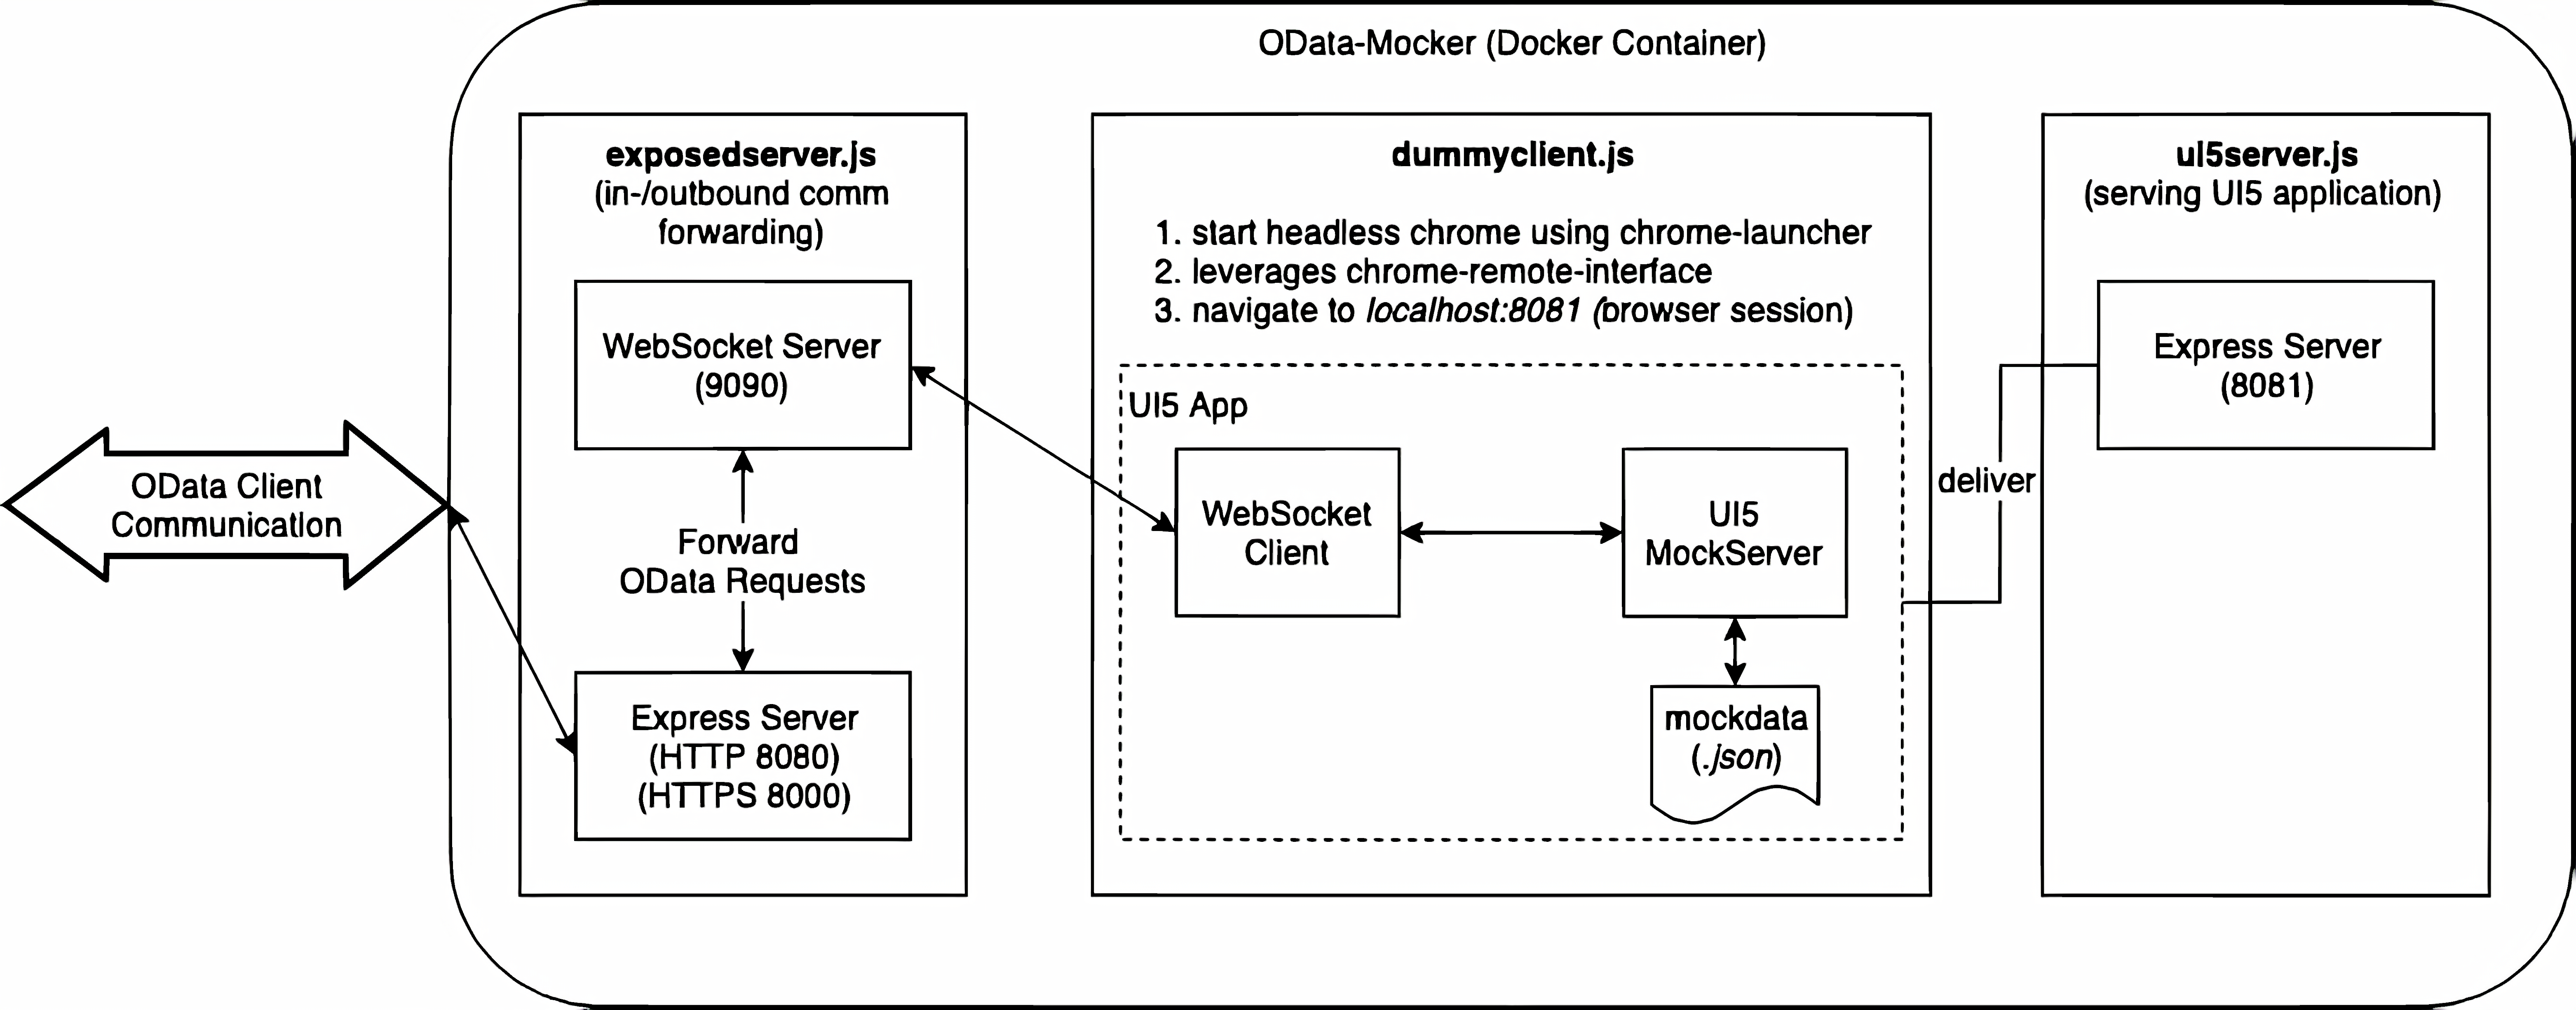
\includegraphics[width=\textwidth]{Bilder/ewm-sim_v1_4x.pdf}
    \caption{Aufbau des ursprünglichen \ac{ewm-sim}}
    \label{fig:ewm-sim-v1}
\end{figure}

\todo{Verweis auf Studentenprojekt, Zusammenarbeit mit Roboter-Anbindung und Unity Simulation}
\chapter{Theoretische Grundlagen}
Im Rahmen der Bearbeitung dieses Projekts wurden einige Technologien eingesetzt, für die hier zunächst Vor- und Nachteile sowie theoretische Grundlagen aufgeführt werden sollen.
Falls eine Entscheidung für eine entsprechende Technologie getroffen werden musste, soll diese anhand der erläuterten Kriterien nachvollziehbar dargelegt werden.

\section{Docker}
\label{docker}
Docker ist eine freie Implementierung des Konzepts der Containervirtualisierung.
Ein sogenannter Docker Container ist plattformübergreifend lauffähig.
Voraussetzung ist lediglich, dass der Docker Daemon auf dem Host-System installiert ist und im Hintergrund ausgeführt wird.
Damit die Container, wie beschrieben, auf allen verbreiteten Betriebssystemen laufen können, setzen sie üblicherweise auf Linux auf.
Somit wird unter Windows das \ac{WSL} genutzt, um die Container auszuführen.
Dies ist eine schlanke Integration des Linux-Kernels in das Windows-Betriebssystem, welche durch Optimierung und Reduktion auf essenzielle Bestandteile den deutlich größeren Overhead von herkömmlicher Virtualisierung erspart.~\cite{wsl}

Kennzeichnend für das Konzept von Docker sind die sogenannten Container.
Diese stellen eine vollständige Zusammenstellung aller Komponenten dar, die eine bestimmte Anwendung zur Ausführung benötigt.
Dadurch ist es sehr einfach, eine Applikation schnell und einheitlich auf einem neuen System zu deployen und dabei direkt alle Abhängigkeiten mitzuinstallieren und richtig zu konfigurieren.~\cite{whatisacontainer}

Docker bietet außerdem eine \enquote{Docker Hub} genannte Plattform an.
Sie bietet eine Möglichkeit, eigene Container Images (also Systemabbilder/Bauanleitungen für eine bestimmte Container-Umgebung) hochzuladen, sowie die von anderen Nutzern hochgeladenen Images zu nutzen.
Diese können zum Beispiel mit einem einzigen Kommandozeilenbefehl heruntergeladen und deployed werden. Sogar als Basis für neue, eigene Images können Images von Docker Hub verwendet werden.~\cite{dockerhub}

Die angestrebte Anwendung als Docker Container zu konzipieren ist neben den oben aufgezählten Vorteilen auch vor allem deshalb naheliegend, weil die erste Version des \ac{ewm-sim} bereits in dieser Form bereitgestellt wurde.
Somit kann bei entsprechender Umsetzung eine identische oder zumindest sehr ähnliche Schnittstelle zur Anbindung an die anderen Softwarekomponenten des Projektes genutzt werden und Umweltfaktoren, die einen reibungslosen Betrieb verhindern würden, sind von vorneherein ausgeschlossen.

\section{Kubernetes}
Wie in \autoref{docker} beschrieben, können mithilfe von Containern leicht Applikationen in einer neuen Umgebung eingerichtet werden.
Kubernetes stellt eine quelloffene Option zur erleichterten und automatisierten Verwaltung von containerisierten Services dar.
Dabei wird von Kubernetes ein deklarativer Ansatz verfolgt.
Das bedeutet: Der Nutzer beschreibt den gewünschten Zustand -- zum Beispiel über Konfigurationsdateien oder die Konsole -- und Kubernetes ermittelt selbstständig die Schritte, die zur Erreichung und Aufrechterhaltung notwendig sind.
Mittels Kubernetes ist es auch möglich, Dienste dynamisch zu skalieren (\dash es werden abhängig von der aktuellen Anzahl der Nutzer eines Dienstes die Ressourcen einer Anwendung entweder erhöht oder wenn möglich gespart) sowie Lastausgleich und Redundanz zwischen verschiedenen Instanzen desselben Services herzustellen.~\cite{Bloß2019, wasistk8s}

Instanzen eines Kubernetessystem werden auch als Cluster bezeichnet.
Ein Cluster besteht aus beliebig vielen Nodes.
Letztere können dabei beliebige Maschinen sein (in der Regel virtuelle Maschinen oder physische Server) auf denen die eigentlichen Anwendungen laufen.
Die Interaktion mit einem Cluster findet über den sogenannten \emph{Kubernetes Master} statt.
Er stellt eine zentrale Verwaltungsstelle dar, mit den Nodes wird praktisch nie direkt interagiert.~\cite{k8skonzepte}

\paragraph{\ac{GKE}}
Kubernetes kann theoretisch auf jedem Heimcomputer installiert und betrieben werden.
Primär findet es jedoch Anwendung im Cloud Computing.
Hierbei können fertige Kubernetes Cluster gemietet werden.
Dies geschieht normalerweise in Form von virtuellen Servern, deren Spezifikationen nach den eigenen Bedürfnissen gewählt werden können, ohne dass selbst Hardware angeschafft werden muss.
Somit ist es möglich, auch für kurze Projekte eine größere Infrastruktur zu deployen oder bei Bedarf und mithilfe der Skalierungsmöglichkeit von Kubernetes mit wenigen Klicks die Ressourcen einer Anwendung beziehungsweise eines Clusters anzupassen.
Weiterhin ist es vorteilhaft, dass nur für die tatsächlich genutzte Rechenzeit und -last gezahlt werden muss.
Google ist mit \ac{GKE} einer der größeren Anbieter von Kubernetes Clustern.~\cite{gke}
Die Entwicklungsabteilung, im Rahmen derer dieses Projekt entwickelt wird, nutzt \ac{GKE}, um dort dynamisch Testumgebungen aufbauen zu können, weshalb ein Grundverständnis von Kubernetes zur Bearbeitung des Projekts von Vorteil ist.
Da die neue Version des \ac{ewm-sim} erneut als Docker erstellt werden soll, sollte sie ebenfalls ohne große Anpassungen der Konfiguration den Platz der alten Implementation im Cloud Cluster einnehmen können.

\section{Node.js}
Seit ihrer ursprünglichen Einführung im Jahre 1995 hat die interpretierte Skriptsprache \emph{JavaScript} rasch an Beliebtheit und Bedeutung gewonnen.
Heutzutage ist sie aus der Web-Entwicklung nicht mehr wegzudenken.
Node.js stellt eine Möglichkeit dar, mithilfe derer JavaScript nicht mehr nur clientseitig im Browser, sondern auch serverseitig ausgeführt werden kann.
Ein großer Vorteil davon liegt darin, dass Web-Entwickler, die bereits viel mit JavaScript arbeiten und dementsprechend damit vertraut sind, nur noch eine Sprache benötigen, um sowohl Frontend als auch Backend zu entwickeln.
Zudem ermöglicht Node.js die parallelisierte Ausführung von Code.
Dies bedeutet, dass ein Web-Server nicht wie traditionell üblich eine Schlange von Anfragen bilden und diese nacheinander beantworten muss, sondern er die Anfragen stattdessen gleichzeitig beantworten kann.

\paragraph{\ac{npm}}
Eine weitere nützliche Funktionalität von Node.js ist der \acl{npm}.
Mit ihm können sehr einfach von der Community erstellte Bibliotheken installiert und in ein Programm eingebunden werden.
Auf diese Weise stehen beispielsweise fertige Frameworks für Web-Server, Unit-Tests oder Logger  mit erweiterter Funktionalität zur Verfügung.
\ac{npm} hilft außerdem bei der strukturierten Verwaltung eines Node.js Projektes.
Er stellt einen Assistenten bereit, um automatisiert eine sogenannte \emph{package.json} zu generieren und auf das Projekt anzupassen.
In ihr werden grundlegende Eigenschaften des Projektes verzeichnet, so zum Beispiel
\begin{itemize}
	\item Name,
	\item Beschreibung,
	\item kennzeichnende Schlüsselwörter,
	\item Lizenzen,
	\item Autoren und Mitwirkende,
	\item Projektwebseite und
	\item Quellcode-Repository.
\end{itemize}
Darüber hinaus werden hier allerdings auch die mit \ac{npm} installierten Pakete inklusive deren Versionsnummer gespeichert, welche wiederum noch in allgemeine Abhängigkeiten und solche, die nur zu Entwicklungszwecken vonnöten sind, untergliedert werden.
Möchte jemand anders das Projekt weiterentwickeln oder ein Deployment durchführen, so können mithilfe von \emph{npm install} im Handumdrehen die entsprechende Laufzeitumgebung dafür geschaffen und Abhängigkeiten befriedigen werden.
Des Weiteren können in der package.json auch Skripte festgelegt werden, die ein einfaches Ausführen, Testen oder Bauen des Projektes, sowie ähnliche Aufgaben ermöglichen.~\cite{package.json}

Die Wahl der zu verwendenden Programmiersprache fiel aus verschiedenen Gründen auf Node.js.
Zunächst muss betrachtet werden, dass die simple Skriptsprache Node.js genau für den Einsatzzweck der serverseitigen Entwicklung konzeptioniert wurde.
Weiterhin ist der SAPUI5 Mock Server selbst in JavaScript geschrieben.
Mithilfe von einigen bereits existierenden \ac{npm}-Modulen ist somit eine sehr einfache Integration mit den bereits vorhandenen Softwarekomponenten möglich.
Auf Docker Hub existiert außerdem eine breite Auswahl an vorgefertigten Images für Node.js-Umgebungen, sodass kein eigenständiges Containerimage von Grund auf hochgezogen werden muss.


\section{Postman}
Bei der Entwicklung eines Web-Servers ist es zu Testzwecken hilfreich, um nicht gar zu sagen unumgänglich, manuell \ac{HTTP}-Requests an diesen schicken zu können.
Ganz grundlegende Anfragen können schon durch einen Web-Browser abgesetzt werden.
Genau dies geschieht beim Aufruf jeder Website.
Diese einfach im Browser abzusetzenden Anfragen stoßen jedoch schnell an ihre Grenzen, weshalb ein Programm mit erweitertem Funktionsumfang benötigt wird, bei dem detailliert Einfluss auf die Parameter von Requests genommen werden kann.
Zunächst kommt ein einfaches und auf vielen Systemen bereits vorinstalliertes Programm in den Sinn, welches einen solchen Funktionsumfang unterstützt: \emph{cURL}.
Das konsolenbasierte Tool bietet allerdings keine Möglichkeit, Requests für spätere Verwendung zu speichern und erfordert mitunter eine komplexe Kombination von Parametern, um das gewünschte Ergebnis zu erzielen.
Anstelle dessen bietet sich Postman an.
Das Programm stellt eine Lösung für alle oben beschriebenen Probleme von cURL dar.
Es bietet eine übersichtliche Oberfläche, um die einzelnen Eigenschaften einer \ac{HTTP}-Request bis ins kleinste Detail zu konfigurieren und ermöglicht es auch, diese zu speichern.
Zur späteren Verwendung gespeicherte Anfragen können in Ordnern organisiert, mit einem Account synchronisiert oder auch als \emph{Collection} im \ac{JSON}-Format zum Austausch mit Mitarbeitern exportiert werden.

\section{Git}
Git ist ein quelloffenes Tool zur Versionsverwaltung, welches ursprünglich von Linus Torvalds zur Entwicklung des Linux-Kernels geschrieben wurde.~\cite{vetter.2019}
Die klassische Bedienung erfolgt über die Kommandozeile.
Mittlerweile gibt es aber auch einige grafische Bedienungsoberflächen, zudem wurde Git direkt in die gängigsten Entwicklungsumgebungen integriert.
Dateien werden in sogenannten Repositories verwaltet, welchen sie durch einen \emph{Commit} hinzugefügt oder in diesen aktualisiert werden.
In einem Repository kann es zudem beliebig viele \emph{Branches} geben, zwischen denen flexibele Wechsel möglich sind.
Die Dateien eines Branches sind unabhängig, \dash es kann zum Beispiel einen Hauptbranch geben, auf dem der stabile Stand des Codes geführt wird und einen, auf dem ein neues Feature entwickelt wird.
Branches können durch \emph{mergen} ineinander überführt werden.
Dies geschieht weitestgehend automatisch, es kann jedoch dabei auch zu Konflikten kommen.
Beispielsweise kann dieser Fall eintreten, wenn dieselbe Zeile einer Datei in beiden Branches bearbeitet wurde.
In dieser Situation muss dann manuell interveniert und der Konflikt beseitigt werden.
Die Zustände des Quellcodes werden zum Zeitpunkt des jeweiligen Commits gespeichert und sind auch nachträglich noch einsehbar.
So können neu hinzugekommene Fehler einfach mittels Rollbacks behoben werden.~\cite{dudler}

\paragraph{GitHub}
Eine große Stärke von Git ist die Möglichkeit zur einfachen Kollaboration.
Hierfür muss ein Repository auf einem Server liegen, von dem aktuelle Änderungen auf den lokalen Rechner heruntergeladen (pull) oder veröffentlicht werden können (push).
GitHub ist einer der größten Anbieter für das Hosting von Git-Repositories und bietet auf der Website noch zahlreiche weitere Möglichkeiten zum Management und der Dokumentation von Projekten.
Hierzu gehören zum Beispiel ein in das Projekt integriertes Wiki, ein Tracker für Probleme (Issues), Statistiken zum Projekt und \emph{Pull Requests} -- ein Feature um Änderungen am Code anderer vorzuschlagen, auf den keine direkten Schreibrechte existieren.~\cite{github.doc}
\ac{EWM} Cloud Robotics ist vollständig quelloffen und wird auf GitHub öffentlich verwaltet.

\section{Travis CI}
\label{sec:travis-desc}
In der professionellen Software-Entwicklung ist es üblich, automatisierte Tests (auch genannt Unittests oder Komponententests) für den Code zu schreiben, um diesen auf korrekte Funktionalität zu überprüfen.
Das Tool Travis CI ist ein Dienst, der für die Durchführung genau dieser Art von Tests konzipiert wurde.
In einer Konfigurationsdatei, die im Projektverzeichnis liegt, werden alle Randbedingungen (wie die genutzte Programmiersprache und das Betriebssystem, auf dem die Tests durchzuführen sind) sowie der genaue Ablauf der Tests festgelegt.
Auch komplexere Abläufe, wie das Kompilieren von mehrschrittigen Builds oder parallelisierte Operationen, können mit Travis CI umgesetzt werden.
Der Dienst wird automatisch aktiv, wenn beispielsweise neuer Code auf einem GitHub-Repository hochgeladen wird.
Die Resultate der Tests können dann entweder auf der Website von Travis CI eingesehen werden oder auch als automatisch generierte Badge im Readme des GitHub-Repositorys oder auf der Projektwebsite eingebunden werden.
Des Weiteren kann eine Benachrichtigung per E-Mail konfiguriert werden, sodass der für das Projekt verantwortliche direkte Rückmeldung darüber erhält, wenn etwas nach einem Update nicht mehr funktionsfähig sein sollte.~\cite{travis}

Travis CI ist eine gute und beliebte Möglichkeit, die Integrität des eigenen Codes zu garantieren.
Allein deshalb schon sollte sie bei diesem Projekt zum Einsatz kommen.
Ein weiterer Vorteil genau dieser Testsuite ist, dass sie bereits für \ac{EWM} Cloud Robotics verwendet wird und somit die Tests des neu entstehenden \ac{ewm-sim}s direkt in das vorhandene Repository eingebunden werden können.

\section{Jira}
Die Abteilung in der \ac{EWM} Cloud Robotics entwickelt wird, arbeitet nach der agilen Projektmanagement-Methodik \emph{Scrum}.
Dort findet Jira als Planungssoftware Verwendung.
Sie erlaubt die Definition von Backlog-Items mit dazugehörigen Sub-Tasks, welche in Sprints verwaltet werden.
In einem aktiven Sprint können mit wenigen Klicks Aufgaben einem Teammitglied zugewiesen oder neue Sub-Tasks erstellt werden.
Die Hauptansicht zur Verwaltung ist in drei Spalten gegliedert, welche den aktuellen Status anzeigen: \emph{To Do}, \emph{In Progress} und \emph{Done}.
Zwischen Spalten hin und her geschoben werden Elemente eines Sprints bequem per Drag and Drop.~\cite{jira}
\chapter{Vorbereitung}
Die Abteilung, in der die Entwicklung von \ac{EWM} Cloud Robotics vorangetrieben wird, legt einen starken Fokus auf innovative Entwicklung.
Aus diesem Grund kommt schon dem Schritt der Vorbereitung besondere Bedeutung zu, da keine Vorgaben hinsichtlich der zu verwendenden Technologien geben wurden, abgesehen von ein paar, die Kompatibilität bedingenden, groben Rahmenbedingung und Hinweisen auf mögliche Ansätze.

% \section{Analyse der bisherigen ewm-sim Implementierung}
% \todo{braucht es das hier überhaupt noch?}

\section{Einarbeitung in und Installation der Basiskomponenten}
\label{sec:einarbeitung}
Node.js und Docker bieten beide eigenständige, geführte Einleitungen an, die den Einsteiger von der Installation bis zu den ersten sichtbaren Lebenszeichen begleiten.
Im Folgenden wird der Aufbau eines kleinen Testprojektes durchlaufen, um an diesem Beispiel die Verwendung der jeweiligen Technologien in Grundzügen zu erläutern.
Beide Tools werden auch gerne in Kombination miteinander eingesetzt.
Dadurch existieren praktischerweise sogar (ebenfalls von beiden Seiten aus) grundlegende Anleitungen, wie eine Node.js-Applikation in einen Docker verpackt werden kann.~\cite{docker-node-hello}

\paragraph{Node.js}
Da Node.js primär für den Einsatz als Webserver vorgesehen und die Erstellung eines Webservices auch Ziel dieser Praxisphase ist, wird hier auch das Testprojekt als Antwort auf eine \ac{HTTP}-Request implementiert (\autoref{code:hello-world.js}).
Hierzu wird zunächst in der ersten Zeile das entsprechende \ac{HTTP}-Modul aus der Standardbibliothek von Node.js geladen.
Anschließend wird der Port gesetzt, unter dem der Service erreichbar sein wird (hier Port 3000).
Als Nächstes wird in Zeile 6 folgende der Server initialisiert.
Mit dem hier vorliegenden Aufruf der Methode \emph{createServer} wird ein Server erstellt, der beim Aufruf jedes Pfades die nachfolgende Callback-Funktion ausführt.
Diese erhält als Parameter eine Request und eine Response.
In den folgenden Zeilen wird zunächst der Statuscode und Inhaltstyp der Response gesetzt und anschließend in Zeile 9 noch ihr Text -- \enquote{Hello, world!} -- festgelegt.
Mit dem Methodenaufruf in Zeile 12 wird der Server gestartet.
\lstinputlisting[
	language=JavaScript,
	label=code:hello-world.js,
	caption=Testserver in Node.js,
	captionpos=b
]{Quellcode/hello-world.js}


\paragraph{Docker}
Nun gilt es, den eben erstellten Server in einen Dockercontainer einzubauen.
Docker werden mithilfe eines sogenannten \emph{Dockerfile}s generiert, welches hier exemplarisch dargestellt ist (\autoref{code:hello-world-docker}).
Auf Docker Hub stehen bereits dutzende Images für den Einsatz als Node.js-Server bereit.~\cite{dockerhub-node}
In der ersten Zeile des Dockerfiles wird mit dem Schlüsselwort \emph{FROM} das Image referenziert, das dem neu Entstehenden als Fundament dienen soll.
Im konkreten Fall heißt das Image \enquote{node}.
Der hinter dem Doppelpunkt folgende Teil wird als Tag bezeichnet.
Mit seiner Hilfe wird eine spezielle Version des Images referenziert, hier \enquote{14-alpine}.
14 steht für die zum Zeitpunkt dieses Projekts aktuelle Node.js-Version.
Wie in der Einführung in die theoretischen Grundlagen bereits erwähnt (siehe \autoref{docker}), bauen Dockercontainer auf Linux-Systemen auf.
Alpine ist eine äußerst leichtgewichtige Linux-Distribution.
Dies bringt zwar unter Umständen einen verringerten Funktionsumfang mit sich, welcher allerdings bei einem stark spezialisiertem Nutzungsfall, wie einem Node-Server innerhalb des Containers, fast nie problematisch wird und theoretisch manuell um die benötigten Pakete erweitert werden kann, was jedoch Arbeit und Detailwissen voraussetzt.
Stattdessen kann durch die Verwendung von Alpine als Basissystem jedoch die Größe des Images um ein Vielfaches reduziert werden.~\cite{Bailey2017}
Ist das Basisimage gewählt, wird im nächsten Schritt das Arbeitsverzeichnis innerhalb des entstehenden Containerimages festgelegt (Zeile 2), in welchem anschließend die Projektdateien eingerichtet werden.
Zunächst werden hierfür die \emph{package.json} und \emph{package-lock.json} Dateien kopiert (Zeile 3) und gemäß den in ihnen enthaltenen Informationen die Abhängigkeiten für das Beispielprojekt im zuvor gewählten Arbeitsverzeichnis installiert (Zeile 4).
Nun werden in Zeile 5 noch die restlichen Dateien in das Image kopiert.
Da die Applikation nun in einem Container laufen wird und diese grundsätzlich unabhängig vom Host-System sind -- auch seitens ihrer Netzwerkfunktionalität -- muss in Zeile 6 noch der im Node-Server gewählte Port für die Weitergabe nach außen hin eingerichtet werden.
Abschließend bleibt nur noch festzulegen, wie der Node-Server gestartet werden kann, was in der siebten Zeile erfolgt.
Durch das \emph{CMD}-Schlüsselwort, welches ein Array an Strings entgegennimmt, wird das benötigte Startkommando hinterlegt, welches beim Start des Containers auf dessen Linux-Kommandozeile ausgeführt wird.
\lstinputlisting[
	language=Docker,
	label=code:hello-world-docker,
	caption=Integration des Testservers in einen Dockercontainer,
	captionpos=b
]{Quellcode/hello-world-Dockerfile}


\paragraph{.dockerignore}
Im vorangegangenen Paragrafen wurden die Node-Module, die als Abhängigkeiten benötigt werden, innerhalb des Containers neu installiert, anstatt aus dem Arbeitsverzeichnis dorthin kopiert zu werden.
Dass dieser Ansatz zu bevorzugen ist, hat verschiedene Gründe.
Zum einen wird so gewährleistet, dass man zum Bauen des Dockerimages aus dem Quellcode keine eigene Installation von Node.js benötigt; um alle relevanten Installationsschritte kümmert sich schließlich das Node-Dockerimage.
Zum anderen ist es auch einfach praktisch, da die Node-Module üblicherweise aus sehr vielen, sehr kleinen Dateien bestehen.
Solche zu kopieren dauert zumeist sehr lange.
Um nun zu verhindern, dass beim Schritt \enquote{den verbliebenen Rest in das Image kopieren} unbeabsichtigt doch der Modul-Ordner oder andere unliebsame Dateien in das Image kopiert wird, kann eine \emph{.dockerignore}-Datei angelegt werden.
Alle in dieser Datei aufgezählten Ordner und Dateien werden dann vom Kopierbefehl ignoriert.~\cite{dockerignore}



\section{Suche nach einer geeigneten Basis}
Kernaufgabe des \ac{ewm-sim} ist die Simulation der \ac{OData}-Schnittstelle eines vollständigen SAP-\ac{EWM}-Systems.
Grundsätzlich existieren viele Wege, über die dies erreicht werden kann.
\ac{OData} ist ein \ac{HTTP}-basiertes Protokoll, welches eine offene Spezifikation darstellt.
Also solche bieten sich grundsätzlich zwei mögliche Vorgehensweisen.
Zum einen bestünde grundsätzlich die Möglichkeit, von Grund auf einen neuen Service zu implementieren, bei dem für sämtliche Requests, die an den Server gestellt werden können, das entsprechende Verhalten und mögliche Antworten abgedeckt werden müssten.
Auf diese Weise wären der Entwicklung die größtmöglichen Freiheiten eingeräumt, sie brächte allerdings auf der anderen Seite auch eine Reihe von potenziellen Problemen und vermeidbaren Fehlern mit sich, da der \ac{OData} Standard relativ umfangreich ist.
Hinzu kommt, dass die Erfahrung in dieser ersten Praxisphase noch stark eingeschränkt war, weshalb dies wahrscheinlich zu einer Überforderung geführt hätte, das Projekt vermutlich nicht in der gesteckten Zeit von zwei Monaten vollständig umsetzbar gewesen wäre und sich somit insgesamt ein alternativer Ansatz empfiehlt.

Diese zweite Möglichkeit besteht in vorgefertigten Modulen, die sich speziell der Aufgabe widmen, eine einfache \ac{OData}-Schnittstelle nachzubilden\footnote{Einige Beispiele sind direkt auf der OData-Website gelistet unter \url{https://www.odata.org/libraries/}.}.
Einige dieser Module finden sich beispielsweise in den \ac{npm}-Repositories, wobei sie je nach Variante einen stark variierenden Funktionsumfang bieten.
Da \ac{OData} ein klar definierter Standard ist, waren die Kernfunktionalitäten dieser Module sehr ähnlich aufgebaut.
Unterschieden haben sie sich vor allem Hinsichtlich der Speicherung der abrufbaren und empfangenen Daten.
Das Format, aus welchem die Services ihre Startdaten lesen, war in allen Fällen \ac{JSON}.
Dies bietet sich vor allem aus dem Grund an, dass es für Menschen leicht les- und schreibbar ist, jedoch auch von Maschinen aufgrund seiner Strukturierung gut verarbeitet werden kann.
Der eben angesprochene Unterschied bestand nun jedoch darin, dass nur wenige der verfügbaren Module in der Lage waren, ihre empfangenen Daten -- welche zur Laufzeit zunächst im Arbeitsspeicher abgelegt werden -- bei der Beendung des Programms persistent zurück in die Quelldateien zu schreiben, damit sich der Server beim nächsten Programmstart wieder in genau dem Zustand befindet, in dem man zuletzt mit ihm gearbeitet hat.
Würde die Implementierung des \ac{ewm-sim} dies beherrschen, so wäre sie schon sehr dicht an einem tatsächlichen \ac{EWM}-System, bei dem die Daten natürlich direkt aus einer Datenbank gelesen und auch dort wieder gespeichert werden.
Auf der anderen Seite entstünden auch Vorteile aus einer flüchtigen Speicherung der Arbeitsdaten.
Da der \ac{ewm-sim} nicht nur zu Kundendemonstrationen verwendet werden soll, sondern auch in der Entwicklung Einsatz finden wird, kann es dort -- etwa für die Fehlersuche -- sehr hilfreich sein, wenn das Serverprogramm bei jedem Start exakt dieselbe Ausgangssituation repräsentiert.
Somit kann durch Veränderung der \ac{JSON}-Dateien auch gezielt ein spezieller Startzustand erzeugt und fixiert werden.

Weiterhin spielen für den \ac{ewm-sim} sogenannte Function Imports eine entscheidende Rolle.
Der Kern der \ac{OData}-Spezifikation umfasst in erster Linie den Abruf sowie die Aktualisierung einzelner Datensätze (Entities) welche wiederum Teil sogenannter Entitysets sind.
Diese Entitysets können ebenfalls angesprochen, gefiltert und hinsichtlich bestimmter Eigenschaften selektiert werden.
Function Imports bieten nun die Möglichkeit, darüber hinaus spezialisierte Anfragen an den Server zu schicken.
So existiert exemplarisch im \ac{ewm-sim} eine Funktion \emph{GetNewRobotWarehouseOrder}, mittels derer sich ein Roboter eine neue \emph{\ac{who}} zuweisen lassen kann.
Auf Function Imports kann in einer Simulation keinesfalls verzichtet werden, da diese, wie am obigen Beispiel anschaulich zu erkennen, für essenzielle Funktionen benötigt werden.
Die verfügbaren Module mussten somit zunächst noch alle auf die Möglichkeit untersucht werden, ob sie die Einrichtung von angepassten Function Imports unterstützen.

Im Laufe der Tests präsentierten sich zwei Kandidaten (\emph{n-odata-server}\footnote{\url{https://github.com/htammen/n-odata-server}} und \emph{varkes}\footnote{\url{https://github.com/kyma-incubator/varkes}}), die zwar sehr angenehm über ein Kommandozeileninterface konfiguriert werden konnten und sogar persistente Speicherung unterstützten, jedoch erfüllte leider keines von beiden die Anforderung der Function Imports.
Von den betrachteten Möglichkeiten konnten diese lediglich im SAP eigenen \emph{Mock Server} eingerichtet werden.

\paragraph{\href{https://github.com/ArnaudBuchholz/node-ui5}{node-ui5}}
Nun kann der Mock Server allerdings, wie in der Einleitung bereits erwähnt, nur in einer \emph{SAPUI5}-Umgebung ausgeführt werden.
Mit dem \ac{npm}-Modul \emph{node-ui5}\footnote{\url{https://github.com/ArnaudBuchholz/node-ui5}} wurde eine Lösung, wie SAPUI5-Tools nicht nur clientseitig, sondern auch auf Node.js-Servern genutzt werden können, bereits vor einiger Zeit von dem kanadischen SAP-Entwickler Arnaud Buchholz entwickelt.
Grundlegend funktioniert dieses Modul ziemlich gut.
Leider bringt es jedoch übliche Probleme solcher in Eigenregie entwickelter \enquote{Ein-Mann-Projekte} mit sich: Die Dokumentation ist nicht besonders ausführlich und zumeist sind andere Arbeitsaufgaben wichtiger, als das Aufspüren und beheben kleinerer Probleme.
Diese Probleme stellten sich, wie zu erwarten, im Laufe des Projekts gelegentlich als kleinere oder größere Schwierigkeiten dar.
Da dieses Modul jedoch das einzig aktuell verfügbare ist, mit dem alle Anforderungen an den \ac{ewm-sim} erfüllt, sowie eine deutliche Verbesserung der Performance erreicht werden können, die eigene Neuerstellung noch deutlich schwieriger geworden und weit über die Möglichkeiten dieser Praxisphase hinaus gegangen wären, wurde es trotzdem als Ausgangspunkt für dieses Projekt gewählt.~\cite{node-ui5-npm, node-ui5-github}
\chapter{Implementierung}
Nachdem die ersten Kontakte mit den beiden Kerntools erfolgt sind und eine geeignete Basis für das Projekt gefunden wurde, gilt es nun, dieses in die Tat umzusetzen.
Wie in \autoref{sec:einarbeitung} kann auch für das richtige Projekt eine Aufteilung der Entwicklung in Erstellung des Servers und anschließende Einbindung in das Containerimage erfolgen, was insbesondere das Testen des Servers während der Entwicklung deutlich vereinfacht und mögliche Fehlerquellen eingrenzt.

\section{Node-Server}
Angesichts dessen, dass der Node-Server im Anschluss lediglich in einen Container eingeschnürt wird, ist die Erstellung des eigentlichen Servers der deutlich größere und wichtigere Bearbeitungsschritt.
Wie bei jedem Projekt liegt auch hier der Einstiegspunkt im Errichten eines Grundgerüsts.
Im konkreten Fall bedeutet das, das node-ui5 Modul erfolgreich in Node.js zu importieren, die richtigen Konfigurationsoptionen dafür zu finden, innerhalb des Moduls den SAP Mock Server anzusteuern und diesen unkonfiguriert für externe Anfragen erreichbar zu machen.
In der Theorie klingt dies einfach.
Allerdings tritt an dieser Stelle sowohl das Problem auf, dass node-ui5 kaum dokumentiert, als auch der Mock Server nicht für solch einen Einsatz vorgesehen ist, wodurch auch die Hilfeseiten von SAP für diesen initialen Schritt nicht sonderlich hilfreich sind.

\subsection{Grundgerüst des Mock Servers}
\label{subsec:foundation}
Für das Node-Projekt wird zunächst die folgende package.json (\autoref{code:basic-ms-package.json}) angelegt.
Hier wird zunächst ein Projektname mit Versionsnummer und Kurzbeschreibung angelegt, sowie in Zeile 5 der Einstiegspunkt für die Applikation definiert.
Die drei, in Zeile 6 folgende festgelegten, Projekt-Abhängigkeiten stellen hier allerdings den primär wichtigen Teil dar.
Das \enquote{body-parser}-Paket wird dafür benötigt, um den Inhalt von Anfragen an den Server sauber verarbeiten zu können.
Mit den hauseigenen Bibliotheken von Node.js ist zwar die Erstellung von Webservern bereits möglich, dieser Prozess wird jedoch vom \enquote{Express}-Framework stark vereinfacht.
Nicht zuletzt wird noch das \enquote{node-ui5}-Modul eingebunden.
Mithilfe der hier definierten Abhängigkeiten, muss nun lediglich noch \emph{npm install} ausgeführt werden und die Implementierung des Mock Servers kann starten.
\lstinputlisting[
	label=code:basic-ms-package.json,
	caption=Package.json für das Grundgerüst (gekürzt),
	captionpos=b,
	firstline=1,
	lastline=10
]{Quellcode/basic-ms/package.json}

Nachfolgend wir in \autoref{code:basic-ms-mockserver.js} der Quellcode der mockserver.js dargestellt.
Beginnend muss node-ui5 eingebunden werden (Zeile 1).
Dies geschieht hier unter Verwendung der mitgelieferten \enquote{factory}, die einige Konfigurationsschritte beim Einbinden direkt übernimmt.
Parameter, die sie dabei berücksichtigen soll, werden in den folgenden 3 Zeilen gesetzt, unter anderem die Variable myApp, als Referenz auf das Verzeichnis, in dem die mockserver.js liegt.
Nachdem node-ui5 in Node eingebunden wurde, wird nun der gesamte folgende Code als Callback-Funktion der Einbindung ausgeführt.
So enthält Zeile 7 bereits SAPUI-Code, welcher weitere SAPUI-Module einbindet (hier MockServer), welche in Zeile 9 einer anschließend automatisch ausgeführten Funktion übergeben werden.

\paragraph{Konfiguration des Mock Servers}
Ab Zeile 10 wird der eigentliche Mock Server initialisiert.
Hierzu wird zunächst in der Variable \emph{ms} ein neues Mock Server Objekt erstellt, welches für den gesamten Subpfad von \enquote{/} zuständig ist.
Zeile 14 folgende teilen dem Mock Server mit, wo er die Daten findet, die er simulieren soll (myApp/mockdata), wie diese strukturiert sind (myApp/metadata.xml) und ob automatisch Platzhalter für fehlende Daten generiert werden sollen.
Zeile 19 bis 21 nehmen schließlich noch die Einstellung vor, dass der Mock Server automatisch antwortet und in diese Antwort eine künstliche Verzögerung einbaut, um die Simulation realistischer zu gestalten, bevor der Mock Server in Zeile 24 gestartet wird.

\paragraph{Externe Freigabe}
Nun läuft der Mock Server zwar und wurde mit Datensätzen versorgt, die er simulieren kann, jedoch ist er noch nicht für Anfragen außerhalb der Node.js-Umgebung erreichbar.
Zu diesem Zweck wird nun ab Zeile 26 noch ein zusätzlicher Webserver mithilfe des Express-Framework eingerichtet.
Zunächst werden hierzu die mit \ac{npm} installierten Module geladen und eine neue Express-Applikation initialisiert.
Das zusätzlich installierte Modul für den body-parser wird nun als Standardparser für Anfragen an den Express-Server konfiguriert (Zeile 30 folgende).
Anschließend wird eine Funktion festgelegt, die für jede Anfrage eines beliebigen Typs (GET, POST, PUT, ...) ausgeführt wird, die an den Express-Server geschickt werden (Zeile 35) und zwar sollen diese alle an den Mock Server weitergeleitet werden.
Der Mock Server ist so implementiert, dass er automatisch alle \ac{AJAX}-Anfragen abfängt.
Somit kann direkt basierend auf den Daten und Parametern der ursprünglichen Anfrage eine solche erstellt werden (Zeile 36-40).
Der \ac{AJAX}-Anfrage wird eine Callback-Funktion übergeben, die ausgeführt wird, wenn die Antwort des Mock Servers auf die Anfrage erfolgt ist.
In dieser werden zunächst sämtliche Header-Daten aus der \ac{AJAX}-Antwort in die Antwort des Express-Servers auf die externe Anfrage kopiert.
Letztere wird anschließend noch mit dem Status-Code der \ac{AJAX}-Response versehen und mit deren Text zurück an den externen Client geschickt (Zeile 41-51).
Übrig bleibt nur noch das Starten des Express-Servers (Zeile 56).
\lstinputlisting[
	label=code:basic-ms-mockserver.js,
	caption=Quellcode des Grundgerüsts (mockserver.js),
	captionpos=b
]{Quellcode/basic-ms/mockserver.js}

\subsection{Function Imports}
Zum aktuellen Zeitpunkt ist es bereits gelungen, einen lauffähigen OData-Service zu errichten, welcher externe Anfragen beantwortet.
Damit dieser nun als neuer \ac{ewm-sim} dienen kann, muss er allerdings zunächst mit den richtigen Mockdaten versorgt werden.
Zu diesem Zweck muss dem Server über die \emph{metadata.xml} mitgeteilt werden, wie die Datenstrukturen und Zusammenhänge zwischen diesen aussehen, die er darstellen soll.
Da der \ac{ewm-sim} eine genaue Nachbildung eines vollständigen \ac{EWM}-Systems sein soll, sind auch die Metadaten mit einem solchen übereinstimmend.
Infolge dessen kann die \emph{metadata.xml} ohne Veränderungen direkt von einem bestehenden \ac{EWM}-System übernommen werden.
Auch die darzustellenden Mockdaten haben noch dieselbe Struktur wie beim \ac{ewm-sim} in der ersten Version.
Um Mock- und Metadaten zu verändern, müssen die jeweiligen Dateien lediglich in die entsprechenden Verzeichnisse gelegt werden, welche in \autoref{subsec:foundation} konfiguriert wurden.
\todo{Code von Meta- und Mockdaten einfügen?}

In den Metadaten werden für den vollständigen Funktionsumfang des Mock Servers jedoch überdies noch Function Imports definiert.
Diese Funktionen stellen Anfragen dar, welche erweiterte Operationen beim Server auslösen, als ausschließlich einen Datensatz zu liefern oder zu manipulieren.
Für die normalen Mockdaten benötigt der Server nicht mehr als die Daten und den entsprechenden Eintrag in den Metadaten.
Bei Function Imports funktioniert das nicht so einfach, hier ist in den Metadaten lediglich festgelegt, dass eine solche Funktion zu existieren hat, auf welche \ac{HTTP}-Methode diese zu reagieren hat, welche Parameter sie entgegennimmt und was sie für einen Wertetyp zurückliefert.
Die eigentliche Funktionalität muss jedoch für jede Funktion einzeln von Hand implementiert werden.
Wie solch eine Implementierung aussieht, soll hier am Beispiel der Funktion \emph{SetRobotStatus} gezeigt werden.

\lstinputlisting[
	language=xml,
	label=code:metadata-setrobotstatus,
	caption=Metadaten der Funktion SerRobotStatus,
	captionpos=b
]{Quellcode/setrobotstatus.xml}

In \autoref{code:metadata-setrobotstatus} ist der für die Funktion relevante Ausschnitt aus der \emph{metadata.xml} zu sehen.
Diesem kann entnommen werden, dass sich die Operation der Funktion auf das \enquote{RobotSet} bezieht und die Funktion auf \ac{HTTP}-POST-Anfragen reagieren soll.
Die Funktion erwartet drei Parameter (Lgnum, Rsrc, Exccode) vom Typ String mit einer jeweils festgelegten, maximalen Länge.

Um jedoch den genauen Ablauf der Funktion im Mock Server implementieren zu können, muss die Implementierung aus dem ABAP-Backend eines richtigen \ac{EWM}-Systems analysiert und in Node.js portiert werden.
Dies ist überdies wichtig, da die importierten Funktionen bestimmte Fehlercodes zurückliefern, die für den Betrieb der Roboter ebenfalls essenziell sind.

\begin{figure}[!ht]
	\centering
	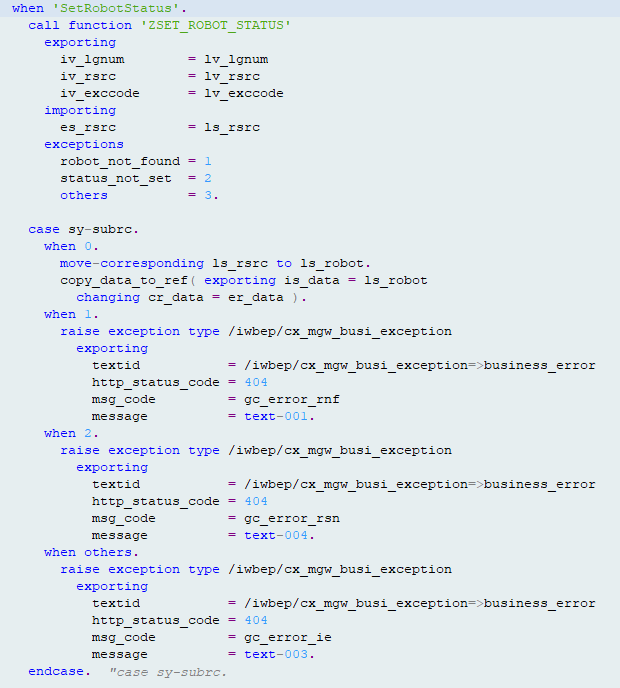
\includegraphics[width=\textwidth]{Bilder/ABAP/2020-12-04 10_20_43-Class Builder Class ZCL_ZEWM_ROBCO_DPC_EXT Display_cut.png}
	\caption{SetRobotStatus im SAP Gateway Service Builder}
	\label{fig:gwse}
\end{figure}

\autoref{fig:gwse} zeigt einen Ausschnitt aus dem \emph{SAP Gateway Service Builder}.
(Vollständige Screenshots werden aus Gründen der Lesbarkeit nicht dargestellt.)
Empfängt der OData-Service den Aufruf von \emph{SetRobotStatus}, ruft er intern im Backend die Funktion \emph{ZSET\_ROBOT\_STATUS} mit den mitgegebenen Parametern auf.
Die Funktion kann zwei klar definierte und eine sonstige Exception zurückliefern.
Diese Exceptions werden Exitcodes zugeordnet und anschließend wird eine Fallentscheidung anhand dieser Rückgabewerte durchgeführt.
Kommt es beispielsweise zur \emph{robot\_not\_found}-Exception, so wird vom OData-Service eine Antwort mit dem \ac{HTTP}-Statuscode \emph{404} zurückgegeben.
Der Nachrichteninhalt wird durch die Konstante \emph{gc\_error\_rnf} festgelegt.
Um von dieser den eigentlichen Wert abzurufen, muss im Class Builder (\autoref{fig:class-builder}) nachgeschlagen werden.
Dort steht zu jeder Konstante (Attribute) der zugehörige Wert des Fehlercodes (Initial Value).

\begin{figure}[!ht]
	\centering
	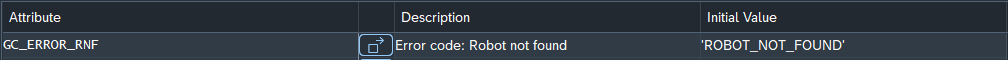
\includegraphics[width=\textwidth]{Bilder/ABAP/2020-12-04 10_22_23-Class Builder_ Display Class ZCL_ZEWM_ROBCO_DPC_EXT_cut.png}
	\caption{Fehlercodes im Class Builder}
	\label{fig:class-builder}
\end{figure}

Nun gilt es die Funktion in Node.js zu implementieren (\autoref{code:set-robot-status-method}).
Hierzu wird zunächst eine Funktion mit dem entsprechenden Namen deklariert, welche die eingehende Anfrage sowie die verwendeten URL-Parameter als Eingabewerte erhält.
Zur einfacheren Verarbeitung wird aus dem zusammenhängenden String von URL-Parametern nun ein Objekt generiert, welches Schlüssel-Wert-Paare besitzt, die entsprechend die URL-Parameter und deren Werten repräsentieren (Zeile 2-8).
Im nächsten Schritt wird überprüft, ob gemäß der übergebenen Parameter ein Roboter im Datensatz existiert, dessen Status gesetzt werden könnte.
Ist dies nicht der Fall, muss eine \emph{ROBOT\_NOT\_FOUND}-Exception zurückgegeben werden.
Die Überprüfung erfolgt über eine Anfrage an das \emph{RobotSet} desselben Servers.
Aus den URL-Parametern wird der anzufragende \ac{URI} generiert und anschließend die Anfrage ausgelöst.
Im Falle von Misserfolg der Anfrage wird die entsprechende Fehlermeldung zurückgegeben, ansonsten kann mit der Ausführung der Funktion fortgefahren werden (vergleiche Zeile 14-34).

In den Metadaten wurde für den Exccode eine maximale Länge festgelegt.
Die Einhaltung dieser muss also überprüft werden, Überschreitung der Länge ist ein Grund zum Abbruch.
Hat der übergebene Code jedoch die richtige Länge, wird erneut eine Anfrage an das servereigene \emph{RobotSet} geschickt.
Dieses Mal wird jedoch keine GET-Request geschickt, sondern mittels PUT-Request die Daten eines bestehenden Datensatzes bearbeitet.
(Durch die vorangegangene Abfrage ist sicher bekannt, dass der angefragte Roboter existiert, sonst würde diese Codestelle gar nicht ausgeführt.)
Als Payload werden schlicht und einfach die URL-Parameter in \ac{JSON}-Form verwendet.
Wird diese Anfrage erfolgreich abgeschlossen, wird die externe Anfrage mit \emph{200 OK} Status quittiert, andernfalls liegt ein weiterer Fehler vor.
Im \emph{SAP Gateway Service Builder} ist nur ein weiterer Fehlertyp vorgesehen.
Da der Roboter an dieser Stelle erwiesenermaßen existiert, liegt nun also der \emph{ROBOT\_STATUS\_NOT\_SET}-Fehler vor.
Dieser Fehler wird ebenfalls zurückgegeben, falls der gewünschte Status länger als die maximal erlaubte Länge sein sollte und ebenfalls in sonstigen Fehlerfällen.

\lstinputlisting[
	label=code:set-robot-status-method,
	caption=Node.js-Implementierung der Funktion SetRobotStatus,
	captionpos=b,
	firstline=1,
	lastline=64
]{Quellcode/setrobotstatus.js}

Nun existiert zwar die Funktion, ihre Existenz ist dem Mock Server jedoch noch nicht bekannt.
Um dies zu ändern, müssen zunächst die bekannten Request Handler des Mock Servers abgerufen werden.
Im Anschluss kann ihnen ein neuer Handler hinzugefügt werden, der per regulärem Ausdruck den Pfad festlegt, über den seine Funktion ausgelöst wird, auf welche Art von \ac{HTTP}-Requests er reagiert und welche Funktion er dann zurückliefern muss.
Abschließend müssen die modifizierten Request Handler noch erneut dem Mock Server bekannt gegeben werden (siehe \autoref{code:request-handler}).

\lstinputlisting[
	label=code:request-handler,
	caption=Hinzufügen des Request Handlers für die Funktion SetRobotStatus,
	captionpos=b,
	firstline=67,
	lastline=73
]{Quellcode/setrobotstatus.js}


\subsection{Authentifizierung}
Die OData-Schnittstelle des \ac{ewm-sim} ist dafür vorgesehen, innerhalb eines Netzwerks freigegeben zu werden.
Im aktuellen Zustand wäre jeder Client in diesem Netzwerk in der Lage, nicht nur Daten von dieser Schnittstelle anzufragen, sondern diese dort auch zu manipulieren, wodurch der ordnungsgemäße Betrieb des \ac{ewm-sim} gestört werden kann.
Aus diesem Grund ist es sinnvoll, eine Authentifizierung einzubauen, die den bislang offenen Zugriff beschränkt.
Eine simple und verbreitete Methode hierfür ist \ac{HTTP}-Authentifizierung, welche, wie der Name schon sagt, direkt in \ac{HTTP} integriert ist.
Um einen Express-Server mit dieser Art der Authentifizierung zu sichern, wird lediglich ein weiteres \ac{npm}-Modul benötigt -- \emph{express-basic-auth}.
Des Weiteren muss die \emph{mockserver.js} um den in \autoref{code:basic-auth} dargestellten Code erweitert werden.
Zunächst wird hier das Modul in den Quellcode importiert (Zeile 1).
Es folgt eine Fallunterscheidung, welche überprüft, ob Zugangsdaten für den Server festgelegt worden sind.
Wie im Umfeld von Containeranwendungen üblich, werden die zu nutzenden Zugangsdaten nicht in den Quellcode integriert, sondern zum Zeitpunkt des Ausführens mittels Umgebungsvariablen festgelegt.
Dies sorgt zum einen dafür, dass für ein Ändern der Zugangsdaten nicht der Quellcode bearbeitet werden muss, zum anderen ist es somit auch unmöglich, den Server mit Standard-Anmeldedaten zu betreiben, was ein großes Sicherheitsmanko darstellen würde.
Wurden keine Zugangsdaten per Umgebungsvariable gesetzt, bricht der Server den Start ab (Zeilen 11-13).
Andernfalls wird in Zeilen 4-8 die \ac{HTTP}-Authentifizierung initialisiert.
Diese nutzt die \emph{safeCompare}-Methode der importierten Bibliothek, welche bereits gegen einige mögliche Arten von Attacken abgesichert ist, und vergleicht Nutzernamen und Passwort, die der Server bei einer Anfrage erhält, mit den in den Umgebungsvariablen festgelegten.
Stimmen beide Wertepaare überein, wird \emph{true} zurückgegeben; die Authentifizierung war erfolgreich.

\lstinputlisting[
	label=code:basic-auth,
	caption=Integration von HTTP-Authentifizierung in den Mock Server,
	captionpos=b
]{Quellcode/basic-auth.js}

\subsection{Unit-Tests}
Da der \ac{ewm-sim} bei der Entwicklung von Produktivsystemen eingesetzt werden soll, ist es von großer Bedeutung, dass er einwandfrei arbeitet.
Um dies zu gewährleisten, ist eine umfassende Überprüfung nach jeder Änderung unerlässlich.
Theoretisch könnten diese Tests händisch durchgeführt werden.
Allerdings hat eine große Software wie der im Zuge dieses Projekts erstellte Mock Server einen so ausgedehnten Funktionsumfang, dass Testungen durch einen Menschen nur stichprobenartig einzelne Funktionen überprüfen könnten.
Unit-Tests oder auch Modultests genannt bieten hingegen eine automatisierte Lösung des Testproblems.
Softwareentwickler müssen bei dieser Variante lediglich einmal solche Tests für jede zu überprüfende Funktionalität ihres Programms schreiben.
Von dort an können die Tests dann eigenständig ausgeführt werden und zeigen im Falle von Fehlern an, wo das tatsächliche Verhalten der Software vom erwarteten Ergebnis abweicht.

Modultests sind in der Softwareentwicklung sehr verbreitet, wodurch praktischerweise für eine populäre Sprache wie Node.js bereits Frameworks zur Erstellung und Durchführung solcher Tests existieren.
Eines der am weitesten verbreiteten ist \emph{Mocha} (verfügbar als \ac{npm}-Modul), mit welchem auch schon die Tests für die erste Version des \ac{ewm-sim} durchgeführt wurden.
Beides in Betracht ziehend fiel auch für die neue Version des \ac{ewm-sim} die Wahl auf Mocha, sodass auch einige bereits bestehende Tests übernommen werden konnten.
Mocha-Tests werden einfach als normale JavaScript-Datei geschrieben und in einem \enquote{test} genannten Ordner im Projektwurzelverzeichnis abgelegt.

\autoref{code:tests} zeigt beispielhaften Inhalt dieser Datei.
Da die Tests automatisiert laufen sollen, muss bei deren Ausführung der Mock Server ebenfalls automatisch gestartet und wieder gestoppt werden, was auch die Konfiguration der Umgebungsvariablen inkludiert und in den ersten drei Zeilen vorgenommen wird.
In den Zeilen 5-7 werden für die Testdurchführung benötigte Bibliotheken geladen.
Dies sind zum einen der Mock Server, eine weitere Bibliothek, die bei der Beschreibung der Testfälle benötigt wird, sowie eine aus dem ersten \ac{ewm-sim} übernommene Hilfsbibliothek, um einfach Anfragen an den Testserver schicken zu können.
Anschließend folgen die eigentlichen Tests.
Testfälle in Mocha sind entfernt einer natürlichen Sprache nachempfunden.
Somit wird ein Testset mit dem Schlüsselwort \emph{\enquote{describe}} (dt. \enquote{beschreibe}) und einer menschenlesbaren Kurzbeschreibung der nachfolgenden Tests eingeleitet (Zeile 9).
Da es für automatisierte Tests üblich ist, dass gewisse Schritte vor und nach der Ausführung eines bestimmten Testfalls durchgeführt werden müssen, bringt Mocha für solches eigene Funktionen (\emph{before} und \emph{after}) mit.
Für den vorliegenden Test erfolgt in der \emph{before}-Funktion der Startvorgang des Mock Servers.
Anschließend folgen die, durch das Schlüsselwort \emph{\enquote{it}} und eine genaue Beschreibung des zu prüfenden Falls gekennzeichneten atomaren Tests.
Diese führen dann die zu testende Interaktion mit dem Server durch und vergleichen das erzielte Resultat (A) mittels der Funktion \emph{\enquote{assert.deepStrictEqual(A, B)}} mit dem erwarteten Resultat (B).
Gleichen sich die Ergebnisse exakt, war der jeweilige Test erfolgreich.

\lstinputlisting[
	label=code:tests,
	caption=Ausschnitt aus den Modultests,
	captionpos=b
]{Quellcode/tests.js}


\section{Erstellung des Dockerimages}
Nachdem der Node-Server vollständig erstellt ist und automatisiert getestet werden kann, besteht der nächste Schritt in der Einbindung in ein Dockerimage.
Der Vorgang ist nur unwesentlich komplizierter als beim in \autoref{sec:einarbeitung} beschriebenen Hello-World-Docker.
Als Besonderheit kommt hier allerdings dazu, dass das Zielimage möglichst klein sein soll.
Aufgrund von Artefakten, die beim Generieren der Node-Module entstehen, muss hier auf ein Multi-Stage-Build zurückgegriffen werden.
\Dash der Prozess der Erstellung des Dockerimages wird in mehrere Abschnitte aufgeteilt.
In \autoref{code:Dockerfile-ewm-sim} ist das entsprechende Dockerfile zu sehen.
Die erste Buildstufe wird in den Zeilen 1-5 durchlaufen.
Hierbei werden die \emph{package.json} sowie die \emph{package-lock.json} in das Arbeitsverzeichnis kopiert und dort mittels \ac{npm} die referenzierten Pakete generiert und installiert.
Anschließend wird die Buildstufe (Zeilen 7-11) gestartet.
Dort werden die restlichen Projektdateien in das eigentliche Containerimage kopiert und anschließend das während der ersten Buildstufe aufgebaute Node-Modulverzeichnis aus dem ersten, temporären Image in das Zielimage kopiert.
Abschließend folgt noch die standardmäßige Freigabe des Ports \emph{8080} für den Webserver (dieser Port kann auch später noch über die Kommandozeile zur Laufzeit angepasst werden) und die Festlegung der Server-Kommandozeile, welche beim Dockerstart ausgeführt werden soll, um auch den Server hochzufahren.

\lstinputlisting[
	label=code:Dockerfile-ewm-sim,
	caption=Dockerfile für den \ac{ewm-sim},
	captionpos=b
]{Quellcode/Dockerfile}


\section{Automatisierte Tests mit Travis CI}
Wie in \autoref{sec:travis-desc} beschrieben, ist Travis CI ein häufig verwendeter Dienst, um Modultests automatisiert ausführen zu lassen, wenn der Code im Online-Repository aktualisiert wird und somit die Integrität der Software zu gewährleisten.
Für dieses Projekt wurde Travis-CI.org (inzwischen zugunsten der neuen Version Travis-CI.com eingestellte Variante) verwendet.
Um Tests für ein GitHub-Repository in Travis CI einzurichten, müssen zwei Dinge erledigt werden.
Zum einen muss eine Registrierung mit dem GitHub-Account, dem das Repository gehört, auf der Website von Travis CI erfolgen.
Hierbei erteilt man dem Dienst Zugriffsberechtigungen für die dem Account zugehörigen Repositories.
Anschließend wird einem von Travis CI eine Liste der auf dem Account gefundenen Repositories angezeigt, in der man mit nur einem weiteren Klick die automatische Verarbeitung für ausgewählte Repositories aktivieren kann.

Als weiterer Schritt muss Travis CI nun noch eine Konfiguration erhalten, wie die Tests für das registrierte Repository durchzuführen sind.
Diese Konfiguration erfolgt mittels der Datei \emph{\enquote{.travis.yml}}, welche im Projektwurzelverzeichnis angelegt wird.
In \autoref{code:travis.yml} ist die Konfigurationsdatei für den \ac{ewm-sim} zu sehen.
Hier wird zunächst festgelegt, in welcher Programmiersprache das Projekt geschrieben wurde und welche Version der Sprache zu verwenden ist (Zeilen 1-3).
Die \emph{install}-Sektion in Zeile 4 definiert, welche Kommandos zur Vorbereitung der Testumgebung ausgeführt werden müssen.
Im konkreten Fall müssen beispielsweise die Abhängigkeiten des Node-Servers installiert werden (Zeile 5).
Es können auch weitere Hook festgelegt werden, so zum Beispiel der in Zeile 6 aufgeführte \emph{after\_success}-Hook, der nach einer erfolgreichen Ausführung des Tests angewandt wird.
Hier wird nach dem Test noch die \enquote{Coverage} (dt. Abdeckung) bestimmt (Zeile 7).
Diese gibt an, wie groß der Anteil des Quellcodes ist, welcher von den Tests abgedeckt wird.
Eine geringe Coverage kann somit darauf hindeuten, dass nicht ausreichend Testfälle definiert wurden, um das korrekte Verhalten der Applikation zu verifizieren.
Ebenfalls in der Konfigurationsdatei festgelegt werden Benachrichtigungen (Zeile 8 fort folgende).
Für den \ac{ewm-sim} wurde dort eine E-Mail-Adresse angegeben, die im Falle von fehlgeschlagenen Tests automatisch benachrichtigt wird.

\lstinputlisting[
	label=code:travis.yml,
	caption=Konfigurationsdatei für automatisierte Tests des \ac{ewm-sim} mit Travis CI,
	captionpos=b
]{Quellcode/travis.yml}


\section{Deployment in \ac{GKE}}
\todo{mach ich das überhaupt noch?..}
\chapter{Performance-Test und Future Work}
Nach Fertigstellung der Neuauflage des \ac{ewm-sim} stellen sich nun natürlich die Fragen: \enquote{Ist es gelungen, den \ac{ewm-sim} im Vergleich zur Vorgängerversion wesentlich zu verbessern? Wenn ja, wie groß ist der Vorsprung?} und \enquote{Wie geht es mit den Ergebnissen weiter? Was kann noch verbessert werden?}.

\section{Locust}
Die einfachste Methode, um die Performance eines Webservices zu bewerten, ist ein sogenannter \emph{Load Test}.
Hierbei wird eine hohe Last in Form von Anfragen an den Service angelegt und währenddessen unter anderem protokolliert, wie lange dieser zur Beantwortung der Anfragen braucht und wie viele Anfragen dabei verloren gehen.
Locust ist eine Python-Bibliothek, um solche Tests ohne großen Aufwand durchführen zu können.~\cite{locust, locust-doc}
Man muss diese hierfür lediglich installieren und in einer kleinen Datei die möglichen Tests beschreiben, die durchgeführt werden sollen.
Zum Vergleich der beiden Service-Implementierungen wurde die in \autoref{code:locustfile.py} dargestellte Locustdatei angelegt.
Die möglichen Anfragen an den Server werden als Methoden der Klasse \emph{ODataUser} implementiert.
Eine Methode wird durch die Annotation \emph{@task(x)} als Test gekennzeichnet.
Über \emph{x} kann hierbei eine Wahrscheinlichkeit angegeben werden, mit der diese Aktion von einem simulierten User ausgeführt wird.
Um die Performance des \ac{ewm-sim} zu testen, werden verschiedene Typen von Anfragen simuliert -- etwa Anzeigen aller Roboter, Erstellen eines neuen Roboters, Löschen eines Roboters oder Anzeigen aller \ac{who}s.


Anschließend kann Locust per Aufruf in der Kommandozeile gestartet werden.
Dies stellt ein kleines Webinterface auf dem lokalen Host zur Verfügung, über welches unter anderem die Anzahl der zu simulierenden Nutzer eingestellt und der eigentliche Load Test gestartet werden kann.

Der Load Test wurde mit 1000 simulierten Nutzern durchgeführt, welche die jeweiligen Services gleichzeitig mit Anfragen kontaktieren.
Das Ergebnis ist überraschend konkret.
Während die ursprüngliche Version des \ac{ewm-sim} durchschnittlich 16,6 Anfragen pro Sekunde beantwortet (\autoref{fig:perf-v1}) sind es bei der neu erstellten Variante rund 104,0 Anfragen pro Sekunde (\autoref{fig:perf-v2}).
Zwar ist die absolute Fehlerrate bei der zweiten Version mit 4,9 Fehlern pro Sekunde deutlich höher als bei der ersten Version mit 0,5 Fehlern pro Sekunde, dies relativiert sich jedoch in Anbetracht des deutlich höheren Durchsatzes der Anfragen.

\begin{figure}[!ht]
	\centering
	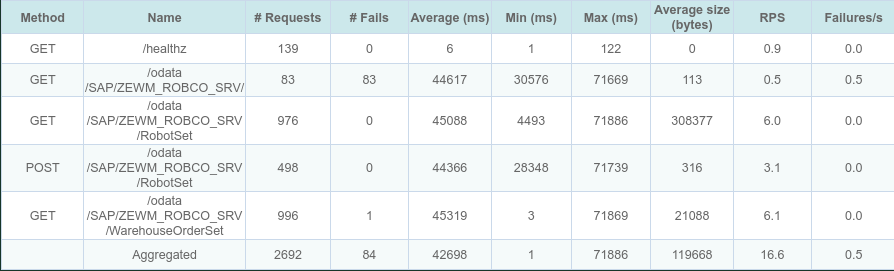
\includegraphics[width=\textwidth]{Bilder/perf-v1.png}
	\caption{Gemessene Performance der ersten Version des \ac{ewm-sim}}
	\label{fig:perf-v1}
\end{figure}

\begin{figure}[!ht]
	\centering
	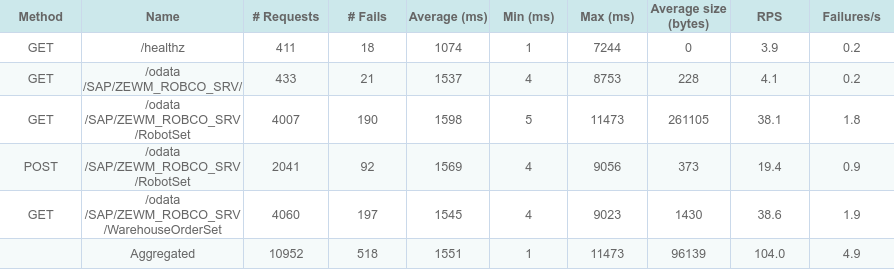
\includegraphics[width=\textwidth]{Bilder/perf-v2.png}
	\caption{Gemessene Performance der zweiten Version des \ac{ewm-sim}}
	\label{fig:perf-v2}
\end{figure}

\section{Future Work}
Trotz der nachweislich besseren Performance kam es bei der längeren Verwendung der neuen Version des \ac{ewm-sim} zu Problemen.
Diese bestehen darin, dass eine Funktionalität endlos neue Daten generiert.
Langfristig führt dies jedoch dazu, dass der Arbeitsspeicher viel zu stark ausgelastet wird, was schlussendlich zu einem Absturz des Simulators führen kann.

Zukünftig ist also auf jeden Fall dieser Missstand noch zu beheben.
Generell war im Rahmen dieser Projektarbeit keine Zeit für ausreichende Langzeittests oder eine Verknüpfung mit den Systemen, die später auf den \ac{ewm-sim} zurückgreifen sollen.
Diese Schritte müssen somit mit gebotener Sorgfalt durchgeführt werden, um auch langfristig einen reibungslosen Betrieb zu gewährleisten.

Des Weiteren wird momentan mit node-ui5 auf ein nicht aktiv entwickeltes und gepflegtes Produkt zurückgegriffen, welches überdies die Komponenten von SAPUI5 in einer Art und Weise verwendet, welche von SAP nie vorgesehen war.
Die aktuelle Implementierung auf Basis von node-ui5 eignet sich zwar schon deutlich besser, als die ursprüngliche, welche innerhalb eines headless Browsers lief, jedoch ist weiterhin ein Overhead vorhandenen.
Aus diesen Gründen sollte langfristig in Betracht gezogen werden, die node-ui5-Basis durch eine eigene OData-Implementierung zu ersetzen.

Allerdings muss bei alldem auch betrachtet werden, dass es sich bei dem \ac{ewm-sim} eben um eine Simulationsumgebung handelt und nicht um ein Produktivsystem.
High Level Performance ist somit nicht kritisch und aufgrund des erheblichen Arbeitsaufwands, welcher mit den vorgeschlagenen Verbesserungen verbunden ist, ist die Umsetzung der meisten davon vermutlich nicht sinnvoll.

Der vollständige Quellcode des Projekts kann unter den Adressen \url{https://github.com/SAP/ewm-cloud-robotics/tree/0353baf3532041cecffcc4243ae52d78a467d5cf/docker/ewm-sim} (Abgabezeitpunkt) und \url{https://github.com/SAP/ewm-cloud-robotics/tree/master/docker/ewm-sim} (aktueller Entwicklungsstand) eingesehen werden.

% ---- Literaturverzeichnis
\cleardoublepage
\renewcommand*{\chapterpagestyle}{plain}
\pagestyle{plain}
\pagenumbering{Roman}                   % Römische Seitenzahlen
\setcounter{page}{\numexpr\value{savepage}+1}
\printbibliography[title=Literaturverzeichnis]

% ---- Anhang
\appendix
%\clearpage
%\pagenumbering{Roman}  % römische Seitenzahlen für Anhang

\newpage
\end{document}
